\section{\textbf{APPENDIX ASTEPI CURVE}} \label{APPENDIX ASTEPI CURVE}


\subsection       {Plot of AstEpi curve
	[\ref  {01-img-Plot of AstEpi curve.pdf} ] }
\label{ssec-01-img-Plot of AstEpi curve.pdf}

\subsection       {AstEpi Radius of Curvature
	[\ref      {02-img-AstEpi Radius of Curvature.pdf}] }
\label{ssec-02-img-AstEpi Radius of Curvature.pdf}

\subsection       {AstEpi Validation in LinuxCNC
	[\ref      {03-img-AstEpi-Validation-in-LinuxCNC.png} ] }
\label{ssec-03-img-AstEpi-Validation-in-LinuxCNC.png}

\subsection     {AstEpi Direction of Travel 3D
	[\ref      {04-img-AstEpi Direction of Travel 3D.pdf} ] }
\label{ssec-04-img-AstEpi Direction of Travel 3D.pdf}

\subsection       {AstEpi First and Second Order Taylors App
	[\ref      {05-img-AstEpi-First-and-Second-Order-Taylors-Approx.pdf}] }
\label{ssec-05-img-AstEpi-First-and-Second-Order-Taylors-Approx.pdf}

\subsection       {AstEpi First minus Second Order Taylors App
	[\ref      {06-img-AstEpi-First-minus-Second-Order-Taylors-Approx.pdf}] }
\label{ssec-06-img-AstEpi-First-minus-Second-Order-Taylors-Approx.pdf}

\subsection       {AstEpi Separate First Second Order Taylors App
	[\ref      {07-img-AstEpi-Separation-First-and-Second-Order-Taylors-Approx.pdf} ] }
\label{ssec-07-img-AstEpi-Separation-First-and-Second-Order-Taylors-Approx.pdf}

\subsection       {AstEpi Separation SAL and SCL
	[\ref      {08-img-AstEpi-Separation-SAL-and-SCL.pdf}] }
\label{ssec-08-img-AstEpi-Separation-SAL-and-SCL.pdf}

\subsection       {AstEpi Chord-error in close view 2 scales
	[\ref      {09-img-AstEpi-Chord-error-in-close-view-2-scales.pdf}] }
\label{ssec-09-img-AstEpi-Chord-error-in-close-view-2-scales.pdf}

\subsection       {AstEpi Four Components Feedrate Limit
	[\ref      {10-img-AstEpi-Four-Components-Feedrate-Limit.pdf} ] }
\label{ssec-10-img-AstEpi-Four-Components-Feedrate-Limit.pdf}

\subsection    {AstEpi FrateCommand FrateLimit and Curr-Frate
	[\ref      {11-img-AstEpi-FrateCommand-FrateLimit-and-Curr-Frate.pdf}] }
\label{ssec-11-img-AstEpi-FrateCommand-FrateLimit-and-Curr-Frate.pdf}

\subsection     {AstEpi FeedRateLimit minus CurrFeedRate
	[\ref      {12-img-AstEpi-FeedRateLimit-minus-CurrFeedRate.pdf} ] }
\label{ssec-12-img-AstEpi-FeedRateLimit-minus-CurrFeedRate.pdf}

\subsection     {AstEpi FC20-Nominal X and Y Feedrate Profiles
	[\ref      {13-img-AstEpi-FC20-Nominal-X-and-Y-Feedrate-Profiles.pdf} ] }
\label{ssec-13-img-AstEpi-FC20-Nominal-X-and-Y-Feedrate-Profiles.pdf}

\subsection     {AstEpi FC20 Nominal Tangential Acceleration
	[\ref      {14-img-AstEpi-FC20-Nominal-Tangential-Acceleration.pdf} ] }
\label{ssec-14-img-AstEpi-FC20-Nominal-Tangential-Acceleration.pdf}

\subsection     {AstEpi FC20 Nominal Rising S-Curve Profile
	[\ref      {15-img-AstEpi-FC20-Nominal-Rising-S-Curve-Profile.pdf} ] }
\label{ssec-15-img-AstEpi-FC20-Nominal-Rising-S-Curve-Profile.pdf}

\subsection     {AstEpi FC20 Nominal Falling S-Curve Profile
	[\ref      {16-img-AstEpi-FC20-Nominal-Falling-S-Curve-Profile.pdf}] }
\label{ssec-16-img-AstEpi-FC20-Nominal-Falling-S-Curve-Profile.pdf}

\subsection       {AstEpi FC10 Colored Feedrate Profile ngcode
	[\ref      {17-img-AstEpi-FC10-Colored-Feedrate-Profile-data_ngcode.png} ] }
\label{ssec-17-img-AstEpi-FC10-Colored-Feedrate-Profile-data_ngcode.png}

\subsection       {AstEpi FC20 Colored Feedrate Profile ngcode
	[\ref      {18-img-AstEpi-FC20-Colored-Feedrate-Profile-data_ngcode.png} ] }
\label{ssec-18-img-AstEpi-FC20-Colored-Feedrate-Profile-data_ngcode.png}

Continue ...\\

\subsection       {AstEpi FC30 Colored Feedrate Profile ngcode
	[\ref      {19-img-AstEpi-FC30-Colored-Feedrate-Profile-data_ngcode.png} ] }
\label{ssec-19-img-AstEpi-FC30-Colored-Feedrate-Profile-data_ngcode.png}

\subsection       {AstEpi FC40 Colored Feedrate Profile ngcode
	[\ref      {20-img-AstEpi-FC40-Colored-Feedrate-Profile-data_ngcode.png} ] }
\label{ssec-20-img-AstEpi-FC40-Colored-Feedrate-Profile-data_ngcode.png}

\subsection       {AstEpi FC10 Tangential Acceleration
	[\ref      {21-img-AstEpi-FC10-Tangential-Acceleration.pdf}] }
\label{ssec-21-img-AstEpi-FC10-Tangential-Acceleration.pdf}

\subsection       {AstEpi FC20 Tangential Acceleration
	[\ref      {22-img-AstEpi-FC20-Tangential-Acceleration.pdf}] }
\label{ssec-22-img-AstEpi-FC20-Tangential-Acceleration.pdf}

\subsection       {AstEpi FC30 Tangential Acceleration
	[\ref      {23-img-AstEpi-FC30-Tangential-Acceleration.pdf}] }
\label{ssec-23-img-AstEpi-FC30-Tangential-Acceleration.pdf}

\subsection       {AstEpi FC40 Tangential Acceleration
	[\ref      {24-img-AstEpi-FC40-Tangential-Acceleration.pdf}] }
\label{ssec-24-img-AstEpi-FC40-Tangential-Acceleration.pdf}

\subsection       {AstEpi FC20 Nominal Separation NAL and NCL
	[\ref      {25-img-AstEpi-FC20-Nominal-Separation-NAL-and-NCL.pdf}] }
\label{ssec-25-img-AstEpi-FC20-Nominal-Separation-NAL-and-NCL.pdf}

\subsection       {AstEpi SAL minus SCL for FC10 FC20 FC30 FC40
	[\ref      {26-img-AstEpi-Difference-SAL-minus-SCL-for-FC10-FC20-FC30-FC40.pdf}] }
\label{ssec-26-img-AstEpi-Difference-SAL-minus-SCL-for-FC10-FC20-FC30-FC40.pdf}


\subsection       {AstEpi FC10 FrateCmd CurrFrate X-Frate Y-Frate
	[\ref      {27-img-AstEpi-FC10-FrateCmd-CurrFrate-X-Frate-Y-Frate.pdf}] }
\label{ssec-27-img-AstEpi-FC10-FrateCmd-CurrFrate-X-Frate-Y-Frate.pdf}

\subsection       {AstEpi FC20 FrateCmd CurrFrate X-Frate Y-Frate
	[\ref      {28-img-AstEpi-FC20-FrateCmd-CurrFrate-X-Frate-Y-Frate.pdf}] }
\label{ssec-28-img-AstEpi-FC20-FrateCmd-CurrFrate-X-Frate-Y-Frate.pdf}

\subsection       {AstEpi FC30 FrateCmd CurrFrate X-Frate Y-Frate
	[\ref      {29-img-AstEpi-FC30-FrateCmd-CurrFrate-X-Frate-Y-Frate.pdf}] }
\label{ssec-29-img-AstEpi-FC30-FrateCmd-CurrFrate-X-Frate-Y-Frate.pdf}

\subsection       {AstEpi FC40 FrateCmd CurrFrate X-Frate Y-Frate
	[\ref      {30-img-AstEpi-FC40-FrateCmd-CurrFrate-X-Frate-Y-Frate.pdf}] }
\label{ssec-30-img-AstEpi-FC40-FrateCmd-CurrFrate-X-Frate-Y-Frate.pdf}

\subsection       {AstEpi FC10 Four Components FeedrateLimit
	[\ref      {31-img-AstEpi-FC10-Four-Components-FeedrateLimit.pdf}] }
\label{ssec-31-img-AstEpi-FC10-Four-Components-FeedrateLimit.pdf}

\subsection       {AstEpi FC20 Four Components FeedrateLimit
	[\ref      {32-img-AstEpi-FC20-Four-Components-FeedrateLimit.pdf}] }
\label{ssec-32-img-AstEpi-FC20-Four-Components-FeedrateLimit.pdf}

\subsection       {AstEpi FC30 Four Components FeedrateLimit
	[\ref      {33-img-AstEpi-FC30-Four-Components-FeedrateLimit.pdf}] }
\label{ssec-33-img-AstEpi-FC30-Four-Components-FeedrateLimit.pdf}

\subsection       {AstEpi FC40 Four Components FeedrateLimit
	[\ref      {34-img-AstEpi-FC40-Four-Components-FeedrateLimit.pdf}]}
\label{ssec-34-img-AstEpi-FC40-Four-Components-FeedrateLimit.pdf}

\subsection       {AstEpi Histogram Points FC10 FC20 FC30 FC40
	[\ref      {35-img-AstEpi-Histogram-Points-FC10-FC20-FC30-FC40.pdf}] }
\label{ssec-35-img-AstEpi-Histogram-Points-FC10-FC20-FC30-FC40.pdf}

\subsection    {AstEpi Table distribution of interpolated points
	[\ref      {tab-AstEpi Table distribution of interpolated points}] }
\label{ssec-tab-AstEpi Table distribution of interpolated points}

\subsection         {AstEpi Table FC10-20-30-40 Run Performance data
	[\ref      {tab-app4-AstEpi-Table-FC10-20-30-40-Run-Performance-data}] }
\label{ssec-tab-app4-AstEpi-Table-FC10-20-30-40-Run-Performance-data}


%% =====================================================
%% =====================================================
\clearpage
\pagebreak

\begin{figure}
	\caption     {Plot of AstEpi curve}
	\label{01-img-Plot of AstEpi curve.pdf}
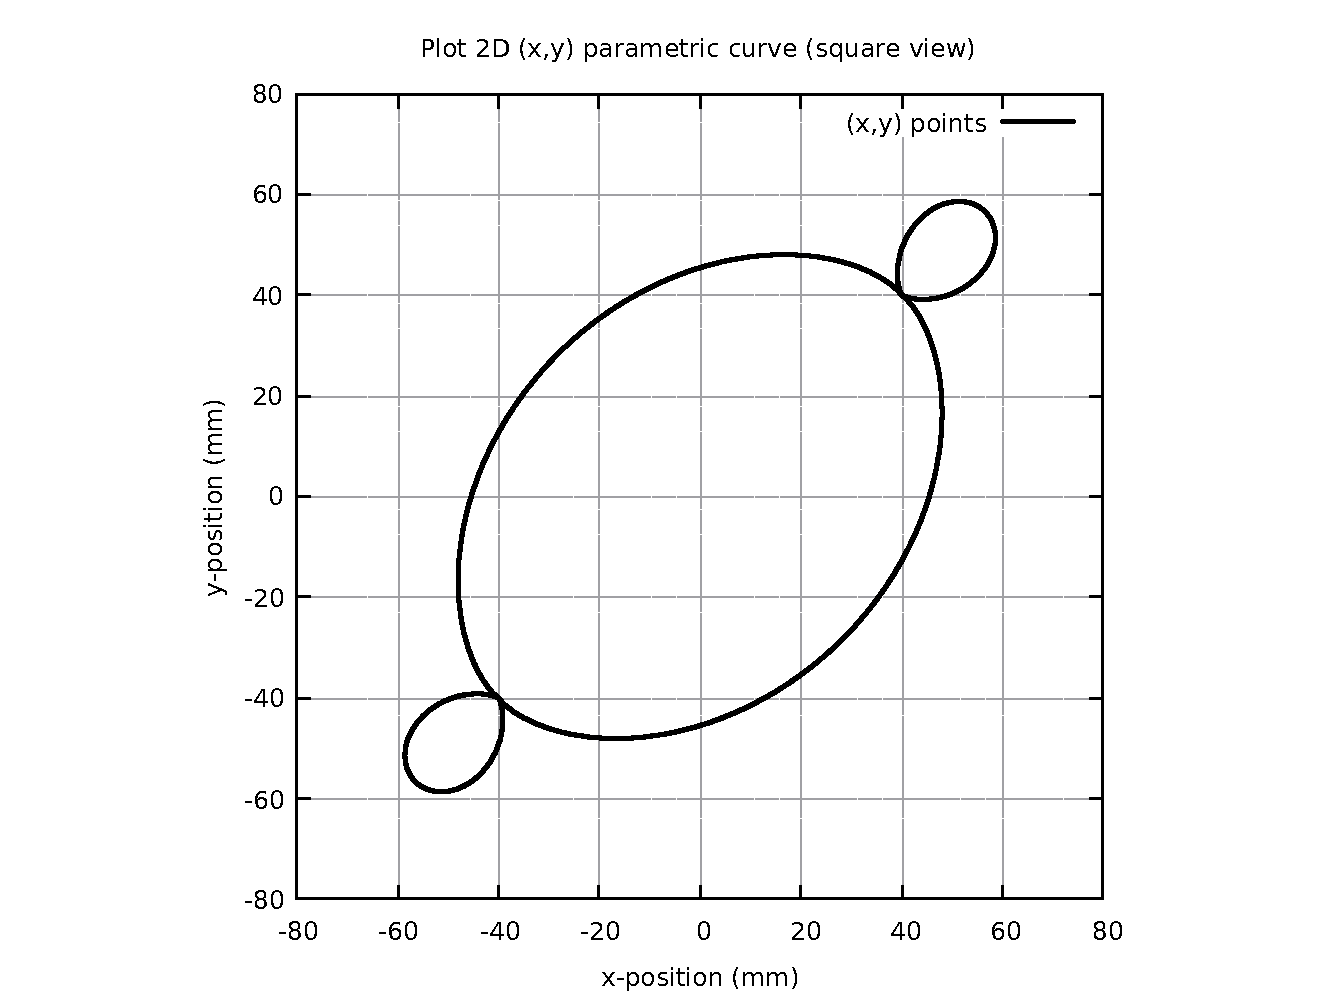
\includegraphics[width=1.00\textwidth]{Chap4/appendix/app-AstEpi/plots/01-img-Plot of AstEpi curve.pdf}
\end{figure}	


\begin{figure}
	\caption     {AstEpi Radius of Curvature}
	\label{02-img-AstEpi Radius of Curvature.pdf}
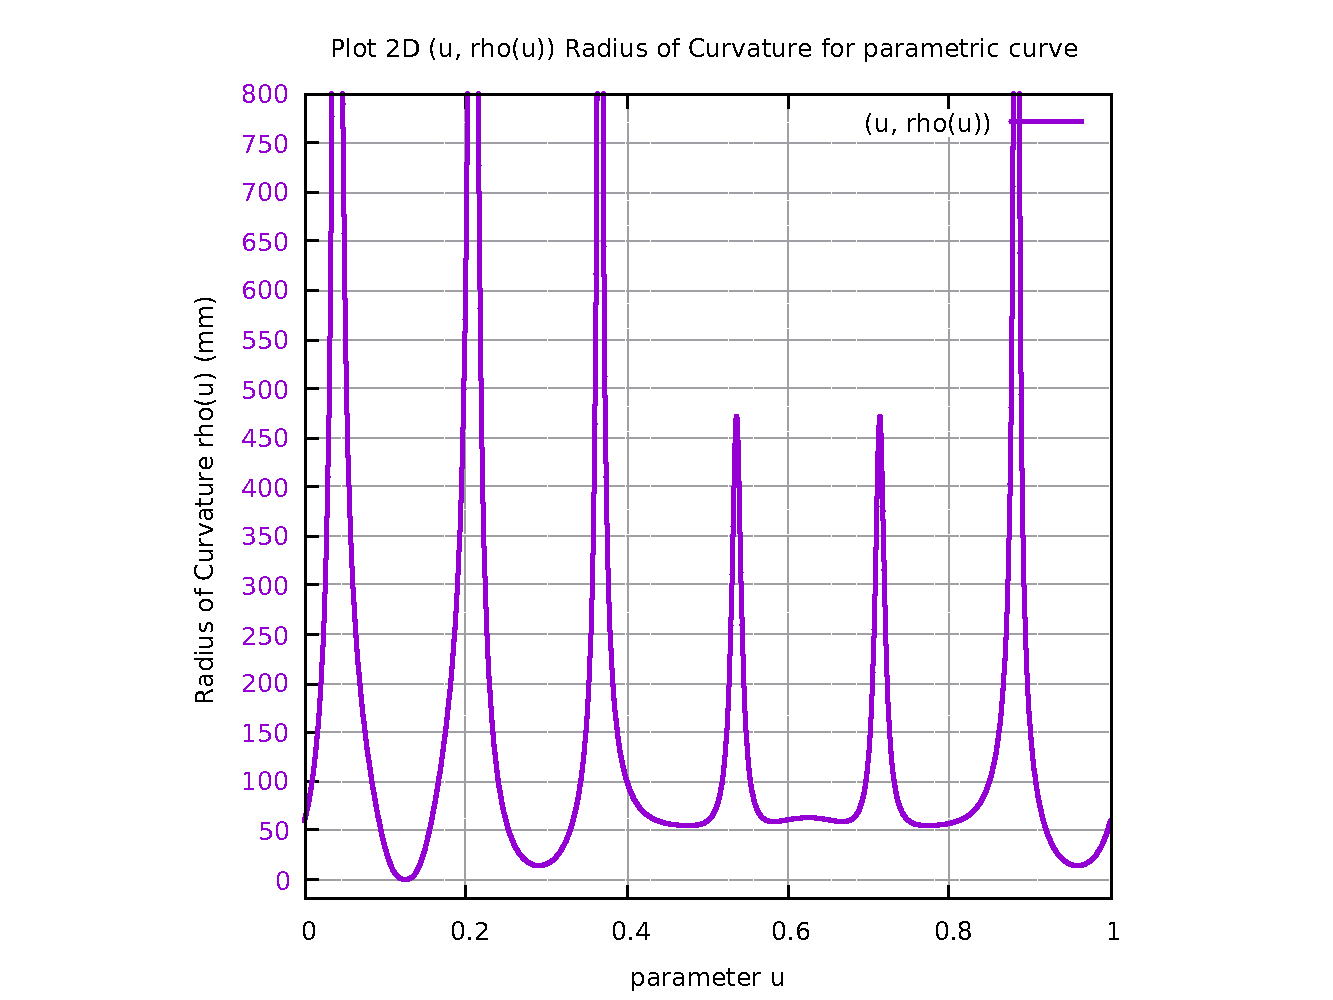
\includegraphics[width=1.00\textwidth]{Chap4/appendix/app-AstEpi/plots/02-img-AstEpi Radius of Curvature.pdf} 
\end{figure}	


%% ==================================================
\clearpage
\pagebreak

\begin{figure}
	\caption     {AstEpi Validation in LinuxCNC}
	\label{03-img-AstEpi-Validation-in-LinuxCNC.png}
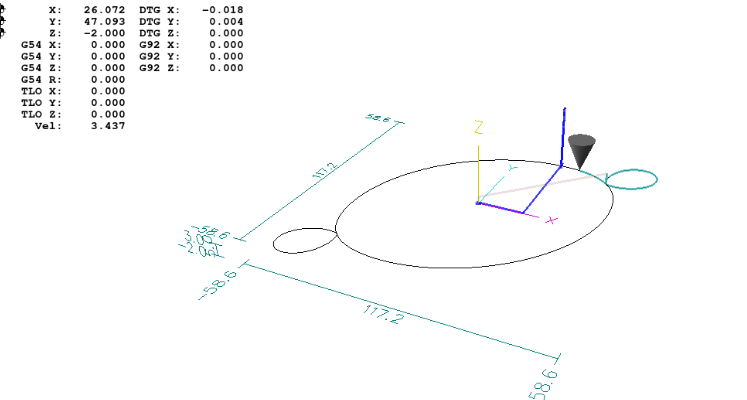
\includegraphics[width=1.00\textwidth]{Chap4/appendix/app-AstEpi/plots/03-img-AstEpi-Validation-in-LinuxCNC.png}
\end{figure}


\begin{figure}
	\caption     {AstEpi Direction of Travel 3D}
	\label{04-img-AstEpi Direction of Travel 3D.pdf}
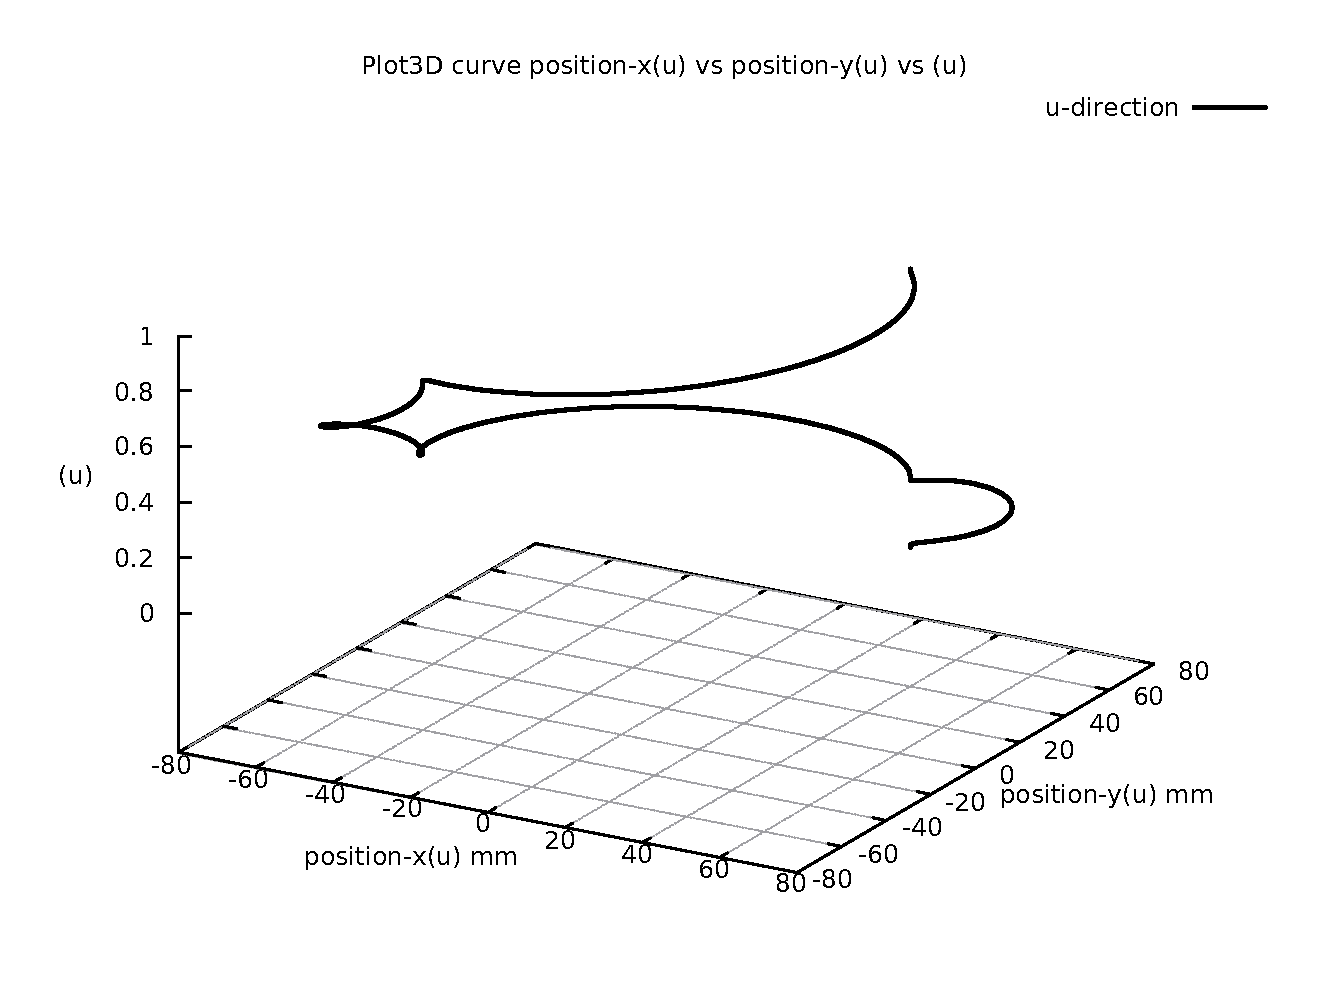
\includegraphics[width=1.00\textwidth]{Chap4/appendix/app-AstEpi/plots/04-img-AstEpi Direction of Travel 3D.pdf}
\end{figure}

%% ==================================================
\clearpage
\pagebreak

\begin{figure}
	\caption     {AstEpi First and Second Order Taylor's Approximation}
	\label{05-img-AstEpi-First-and-Second-Order-Taylors-Approx.pdf}
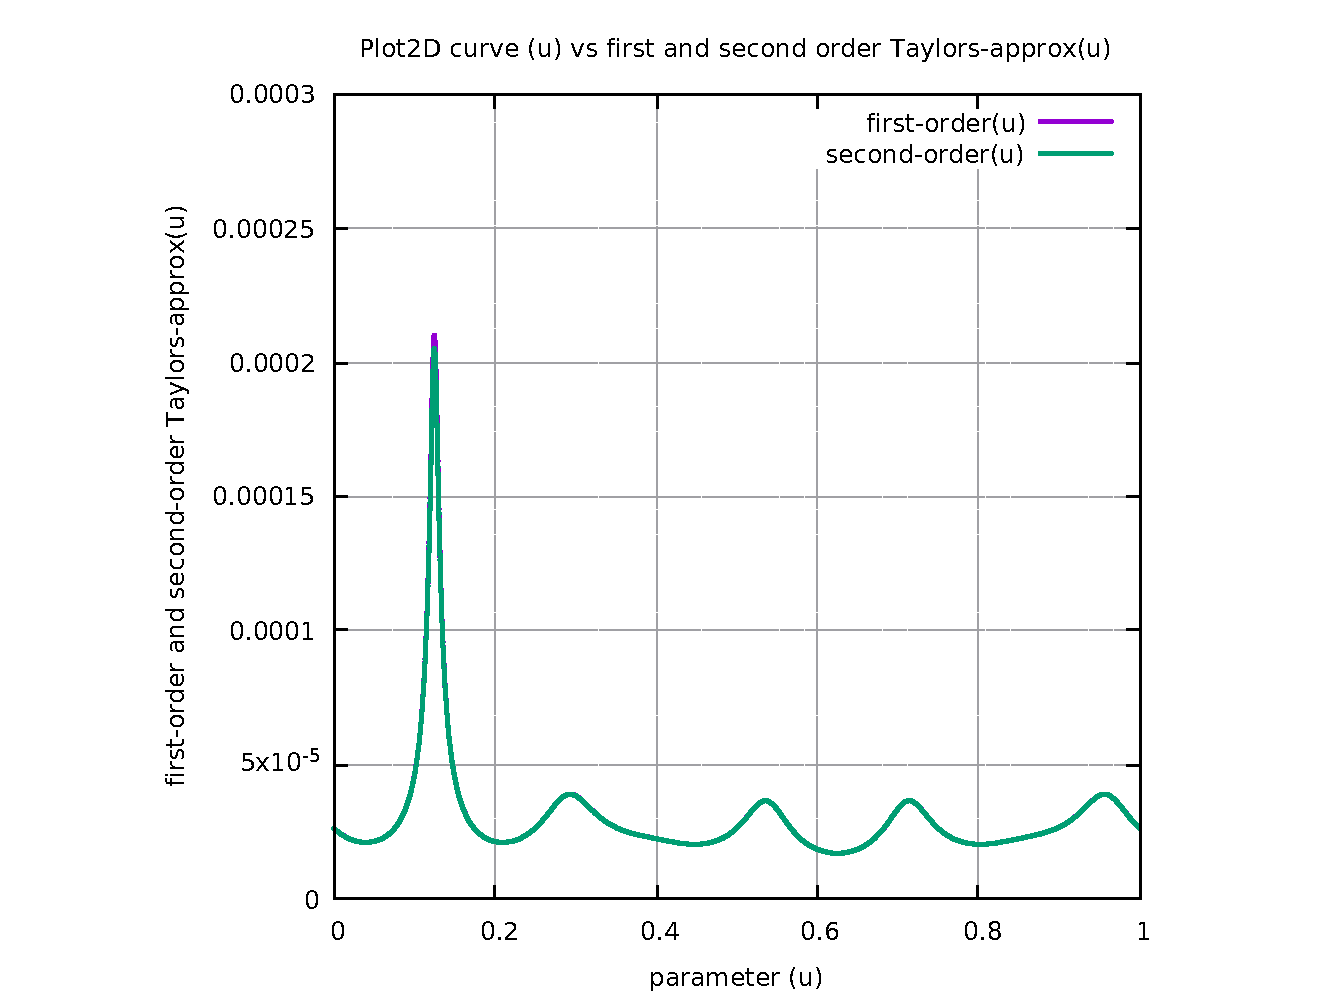
\includegraphics[width=1.00\textwidth]{Chap4/appendix/app-AstEpi/plots/05-img-AstEpi-First-and-Second-Order-Taylors-Approx.pdf}
\end{figure}


\begin{figure}
	\caption     {AstEpi First minus Second Order Taylor's Approximation}
	\label{06-img-AstEpi-First-minus-Second-Order-Taylors-Approx.pdf}
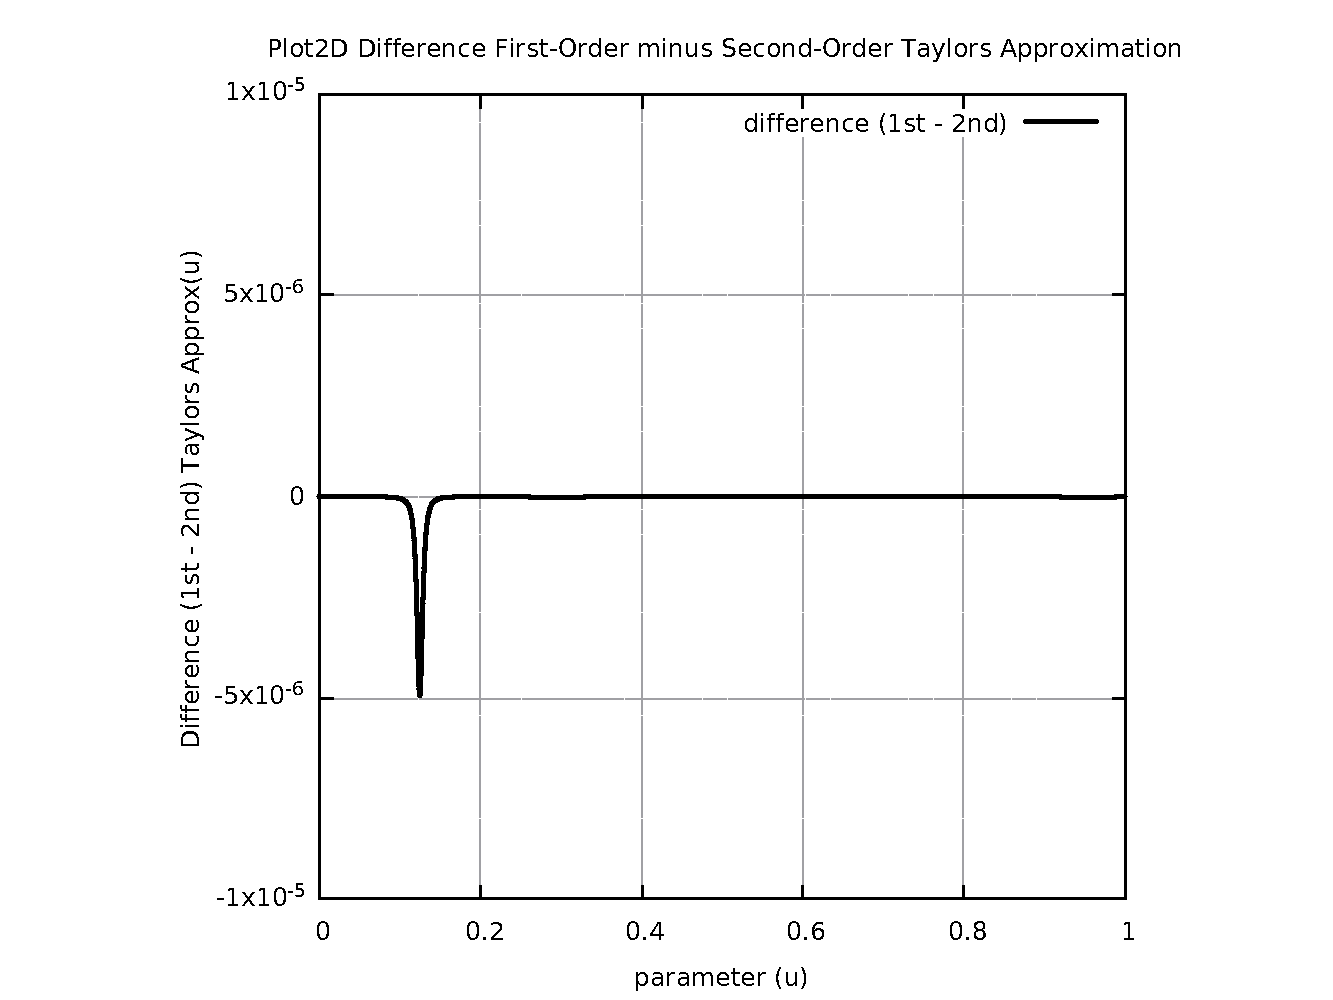
\includegraphics[width=1.00\textwidth]{Chap4/appendix/app-AstEpi/plots/06-img-AstEpi-First-minus-Second-Order-Taylors-Approx.pdf}
\end{figure}

%% ==================================================
\clearpage
\pagebreak

\begin{figure}
	\caption     {AstEpi Separation First and Second Order Taylor's Approximation}
	\label{07-img-AstEpi-Separation-First-and-Second-Order-Taylors-Approx.pdf}
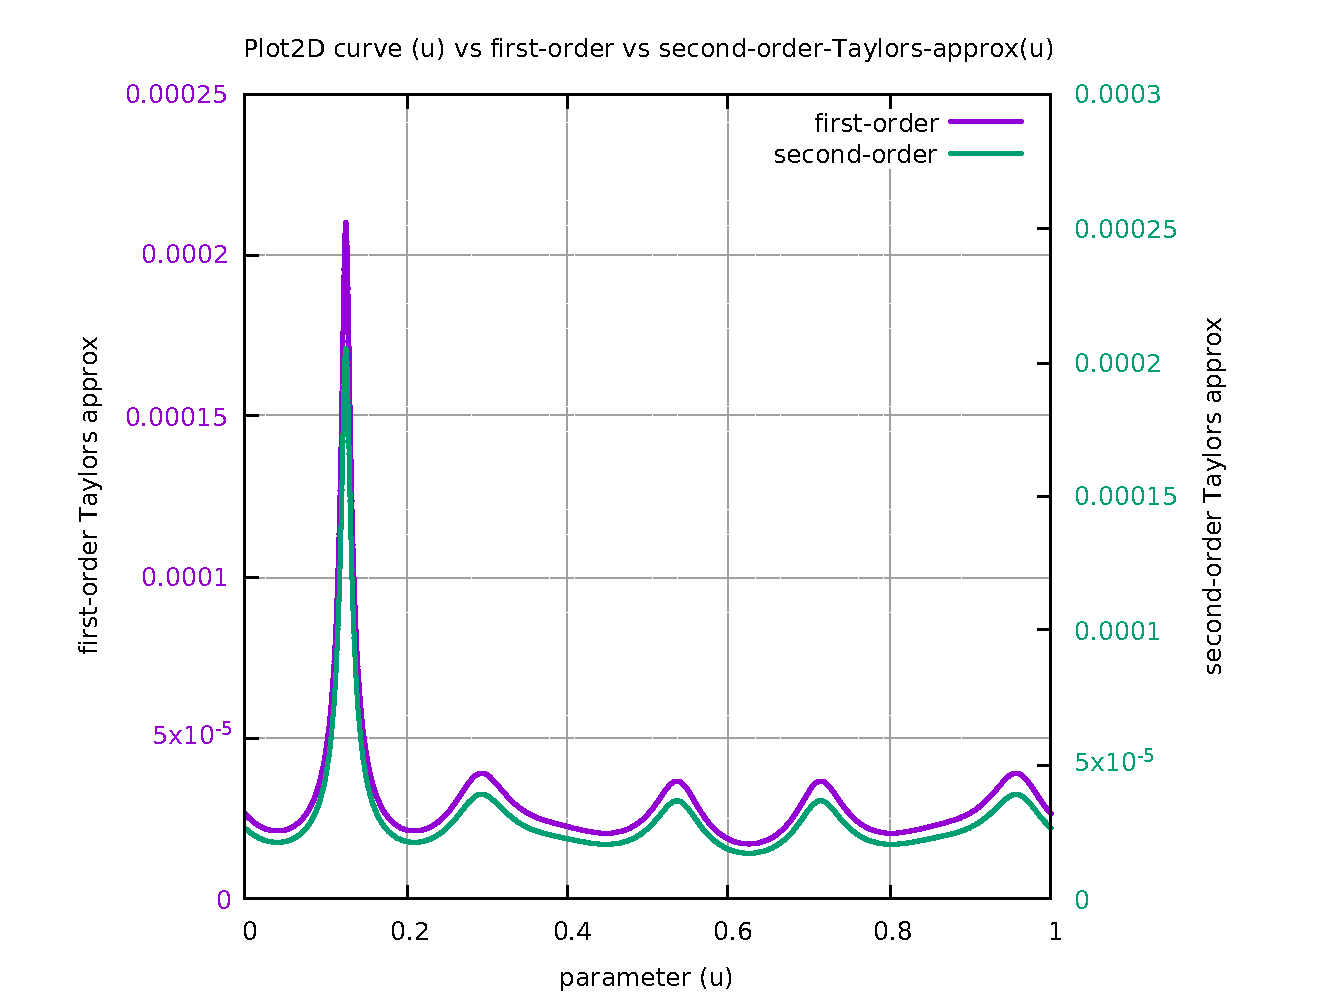
\includegraphics[width=1.00\textwidth]{Chap4/appendix/app-AstEpi/plots/07-img-AstEpi-First-and-Second-Order-Taylors-Approx.pdf}
\end{figure}


\begin{figure}
	\caption     {AstEpi Separation SAL and SCL}
	\label{08-img-AstEpi-Separation-SAL-and-SCL.pdf}
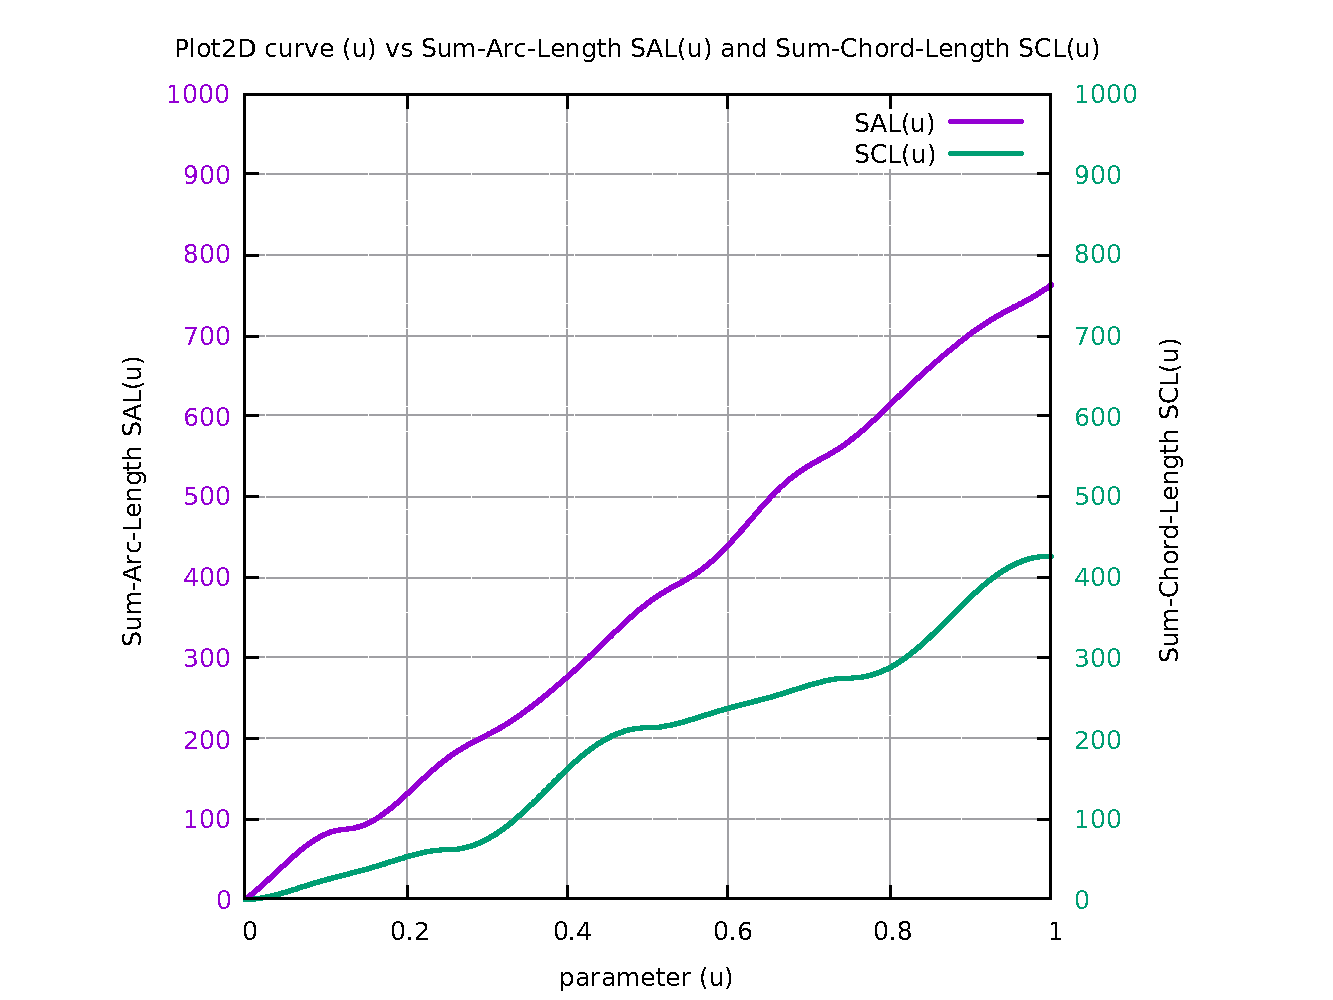
\includegraphics[width=1.00\textwidth]{Chap4/appendix/app-AstEpi/plots/08-img-AstEpi-Separation-SAL-and-SCL.pdf}
\end{figure}

%% ==================================================
\clearpage
\pagebreak

\begin{figure}
	\caption     {AstEpi Chord-error in close view 2 scales}
	\label{09-img-AstEpi-Chord-error-in-close-view-2-scales.pdf}
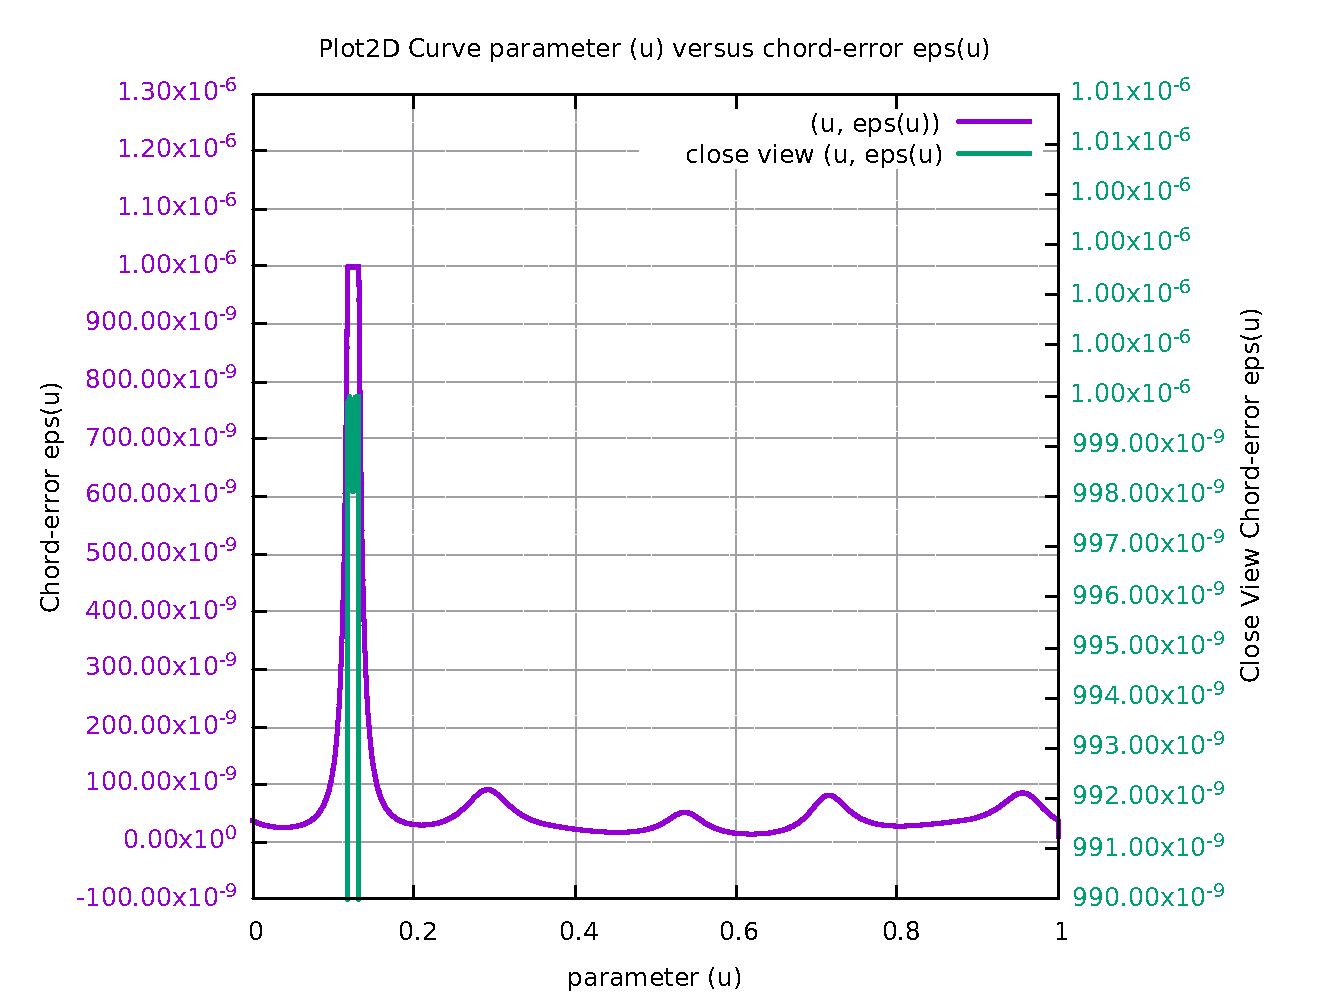
\includegraphics[width=1.00\textwidth]{Chap4/appendix/app-AstEpi/plots/09-img-AstEpi-Chord-error-in-close-view-2-scales.pdf}
\end{figure}

\begin{figure}
	\caption     {AstEpi Four Components Feedrate Limit}
	\label{10-img-AstEpi-Four-Components-Feedrate-Limit.pdf}
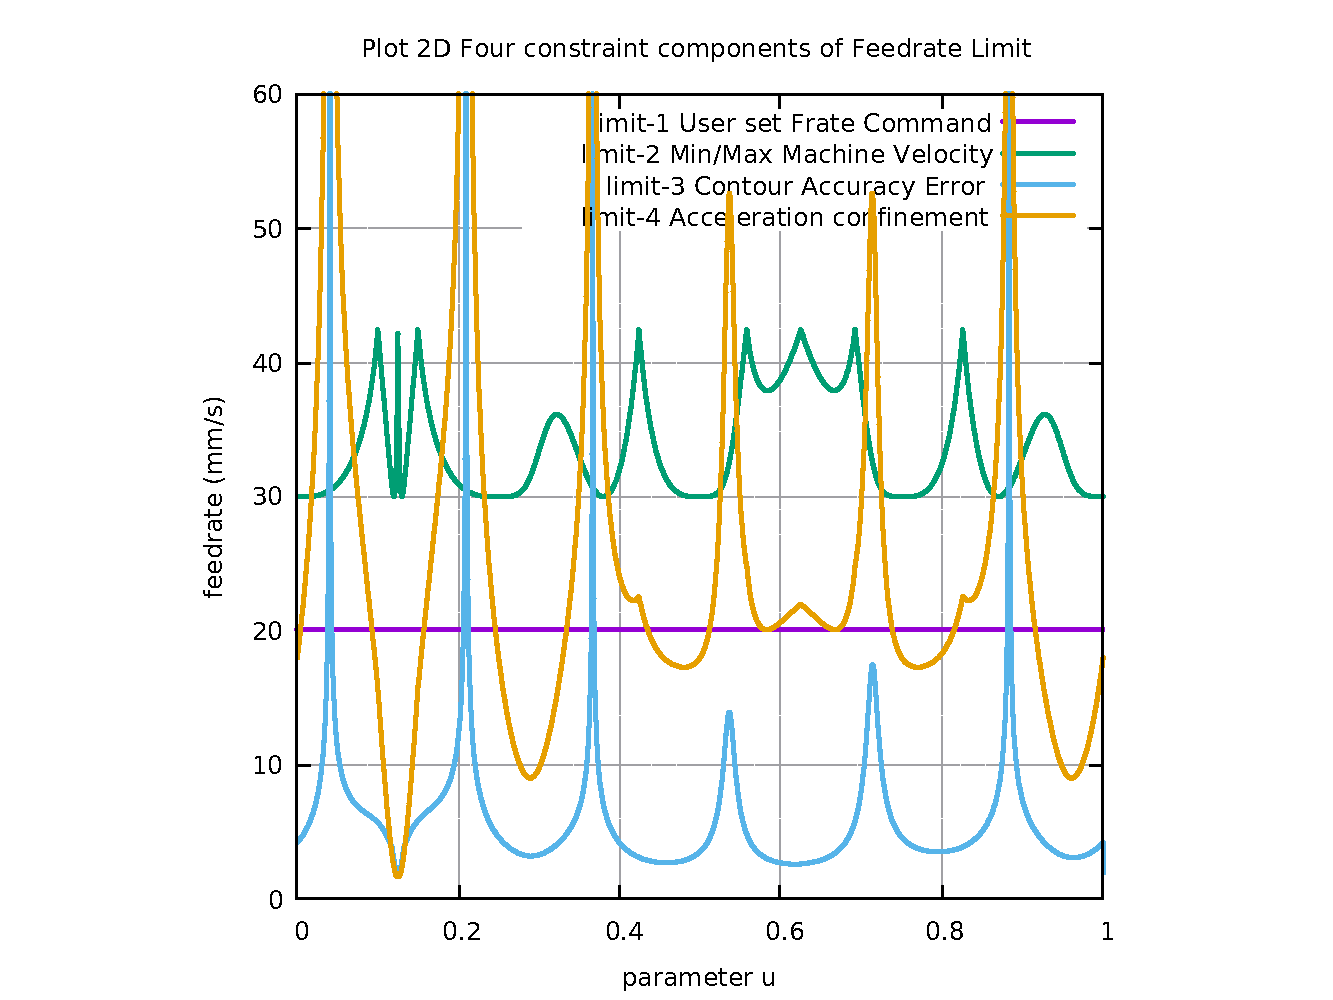
\includegraphics[width=1.00\textwidth]{Chap4/appendix/app-AstEpi/plots/10-img-AstEpi-Four-Components-Feedrate-Limit.pdf}
\end{figure}

%% ==================================================
\clearpage
\pagebreak

\begin{figure}
	\caption     {AstEpi FrateCommand FrateLimit and Curr-Frate}
	\label{11-img-AstEpi-FrateCommand-FrateLimit-and-Curr-Frate.pdf}
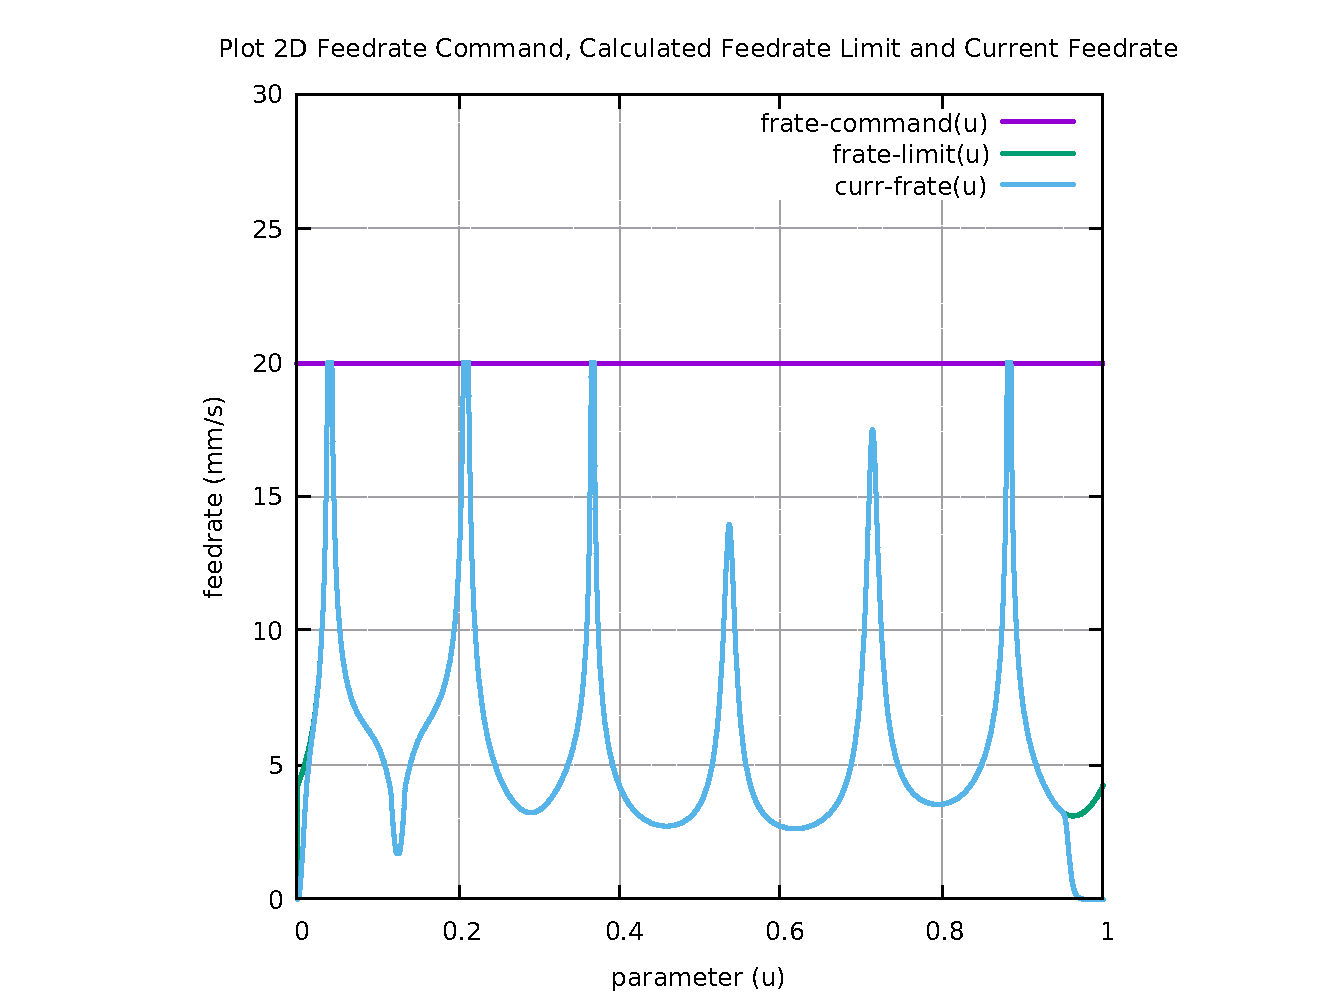
\includegraphics[width=1.00\textwidth]{Chap4/appendix/app-AstEpi/plots/11-img-AstEpi-FrateCommand-FrateLimit-and-Curr-Frate.pdf}
\end{figure}

\begin{figure}
	\caption     {AstEpi FeedRateLimit minus CurrFeedRate}
	\label{12-img-AstEpi-FeedRateLimit-minus-CurrFeedRate.pdf}
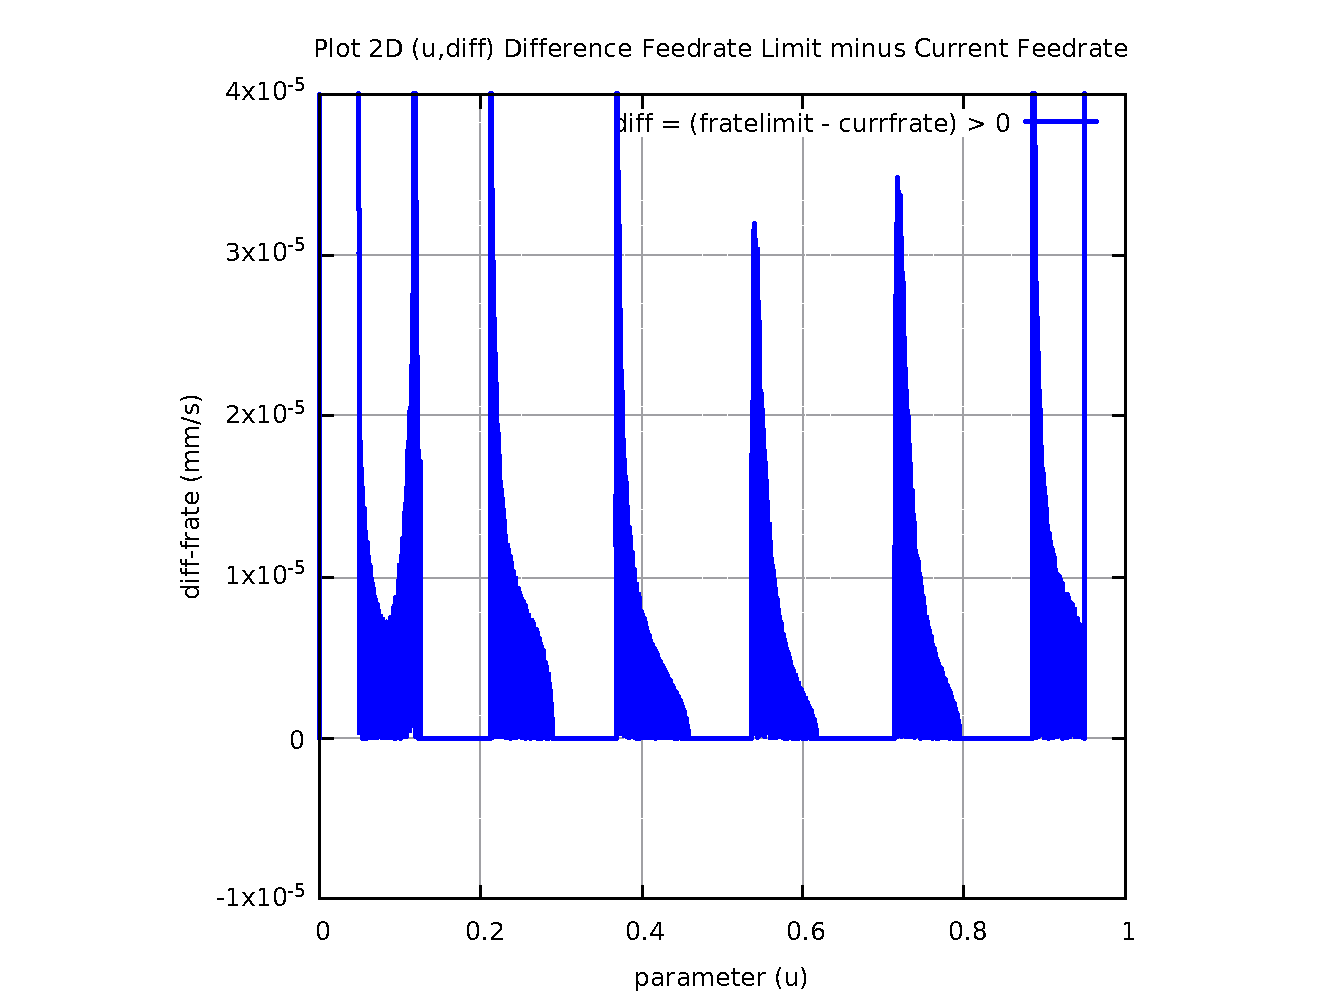
\includegraphics[width=1.00\textwidth]{Chap4/appendix/app-AstEpi/plots/12-img-AstEpi-FeedRateLimit-minus-CurrFeedRate.pdf}
\end{figure}

%% ==================================================
\clearpage
\pagebreak

\begin{figure}
	\caption     {AstEpi FC20-Nominal X and Y Feedrate Profiles}
	\label{13-img-AstEpi-FC20-Nominal-X-and-Y-Feedrate-Profiles.pdf}
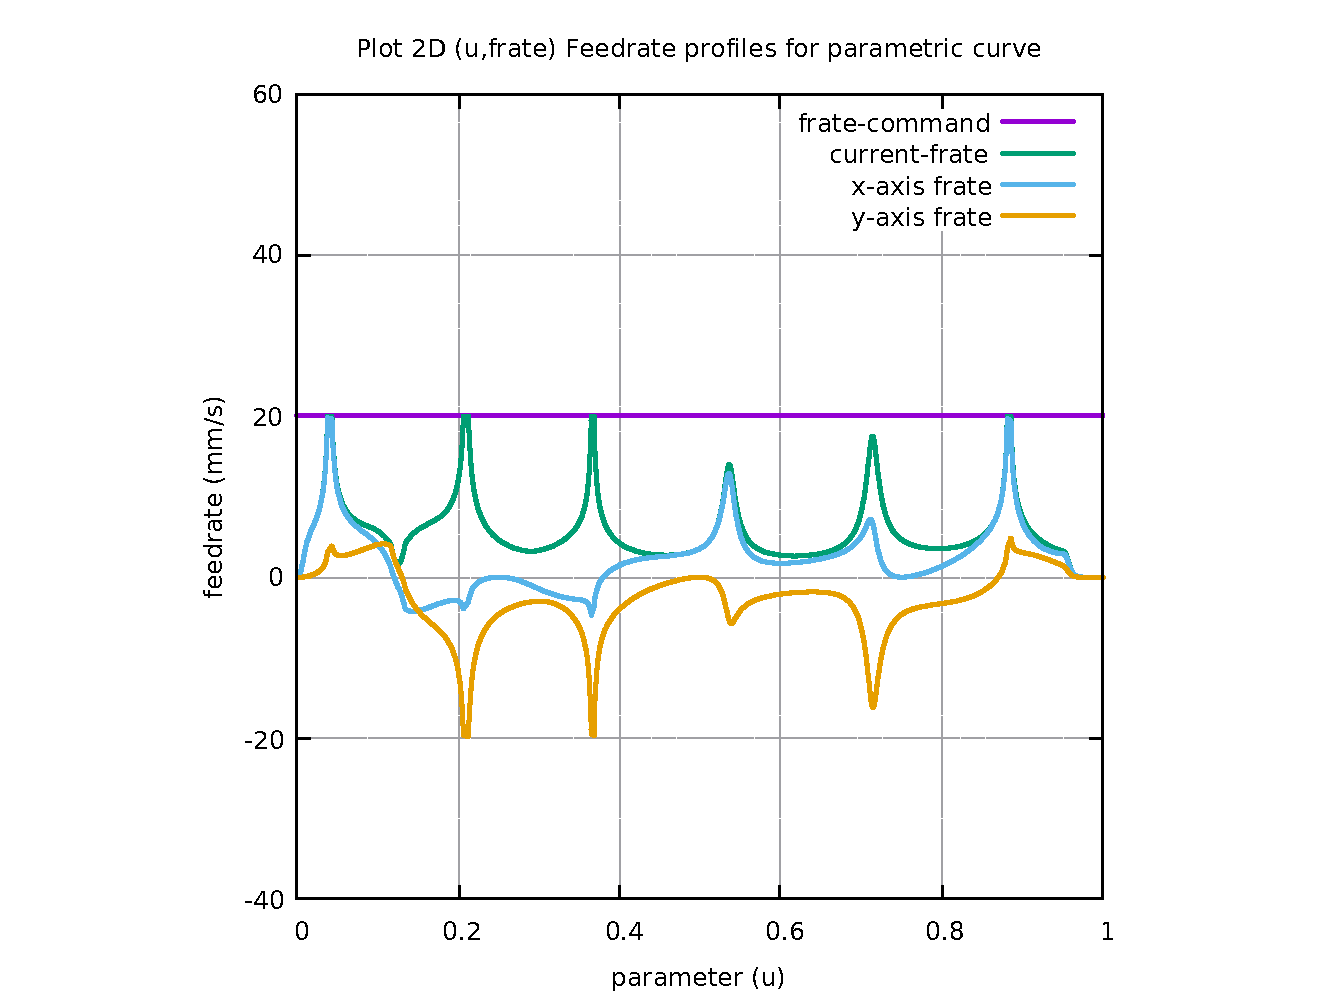
\includegraphics[width=1.00\textwidth]{Chap4/appendix/app-AstEpi/plots/13-img-AstEpi-FC20-Nominal-X-and-Y-Feedrate-Profiles.pdf}
\end{figure}


\begin{figure}
	\caption     {AstEpi FC20 Nominal Tangential Acceleration}
	\label{14-img-AstEpi-FC20-Nominal-Tangential-Acceleration.pdf}
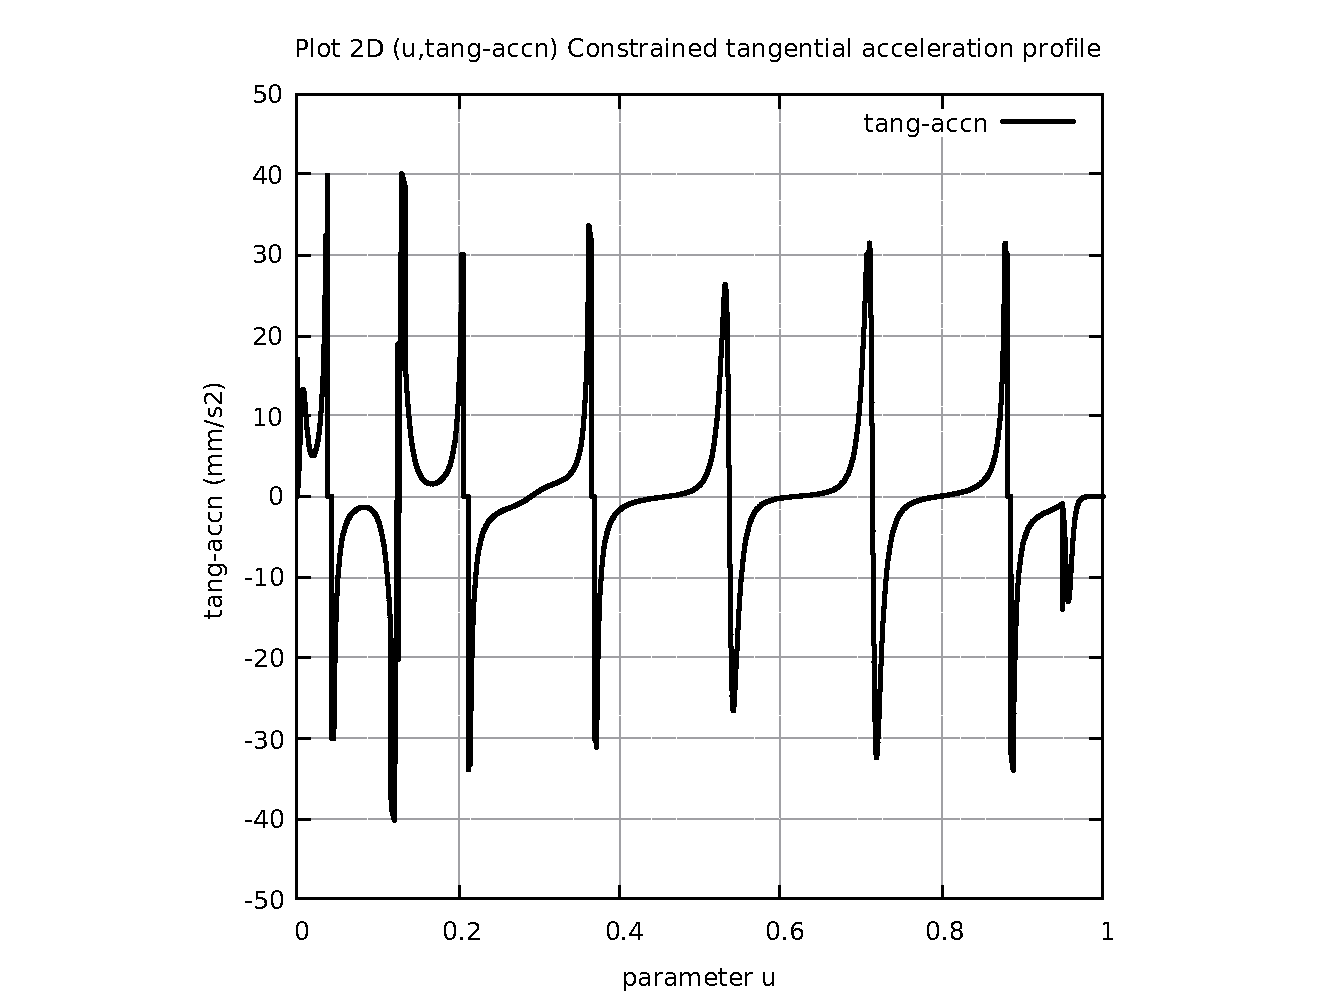
\includegraphics[width=1.00\textwidth]{Chap4/appendix/app-AstEpi/plots/14-img-AstEpi-FC20-Nominal-Tangential-Acceleration.pdf}
\end{figure}

%% ==================================================
\clearpage
\pagebreak

\begin{figure}
	\caption     {AstEpi FC20 Nominal Rising S-Curve Profile}
	\label{15-img-AstEpi-FC20-Nominal-Rising-S-Curve-Profile.pdf}
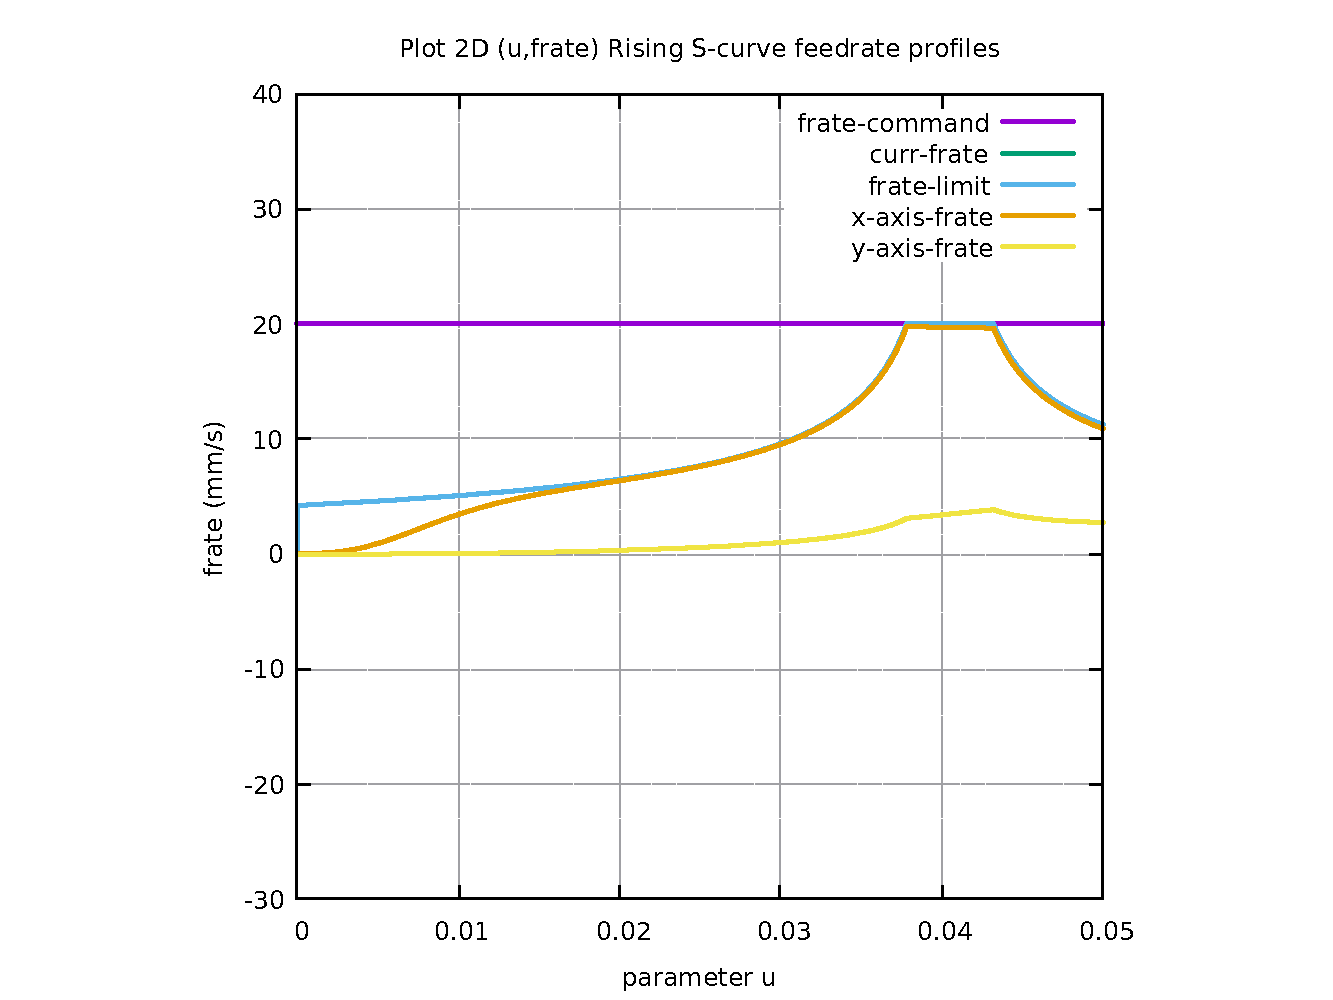
\includegraphics[width=1.00\textwidth]{Chap4/appendix/app-AstEpi/plots/15-img-AstEpi-FC20-Nominal-Rising-S-Curve-Profile.pdf}
\end{figure}


\begin{figure}
	\caption     {AstEpi FC20 Nominal Falling S-Curve Profile}
	\label{16-img-AstEpi-FC20-Nominal-Falling-S-Curve-Profile.pdf}
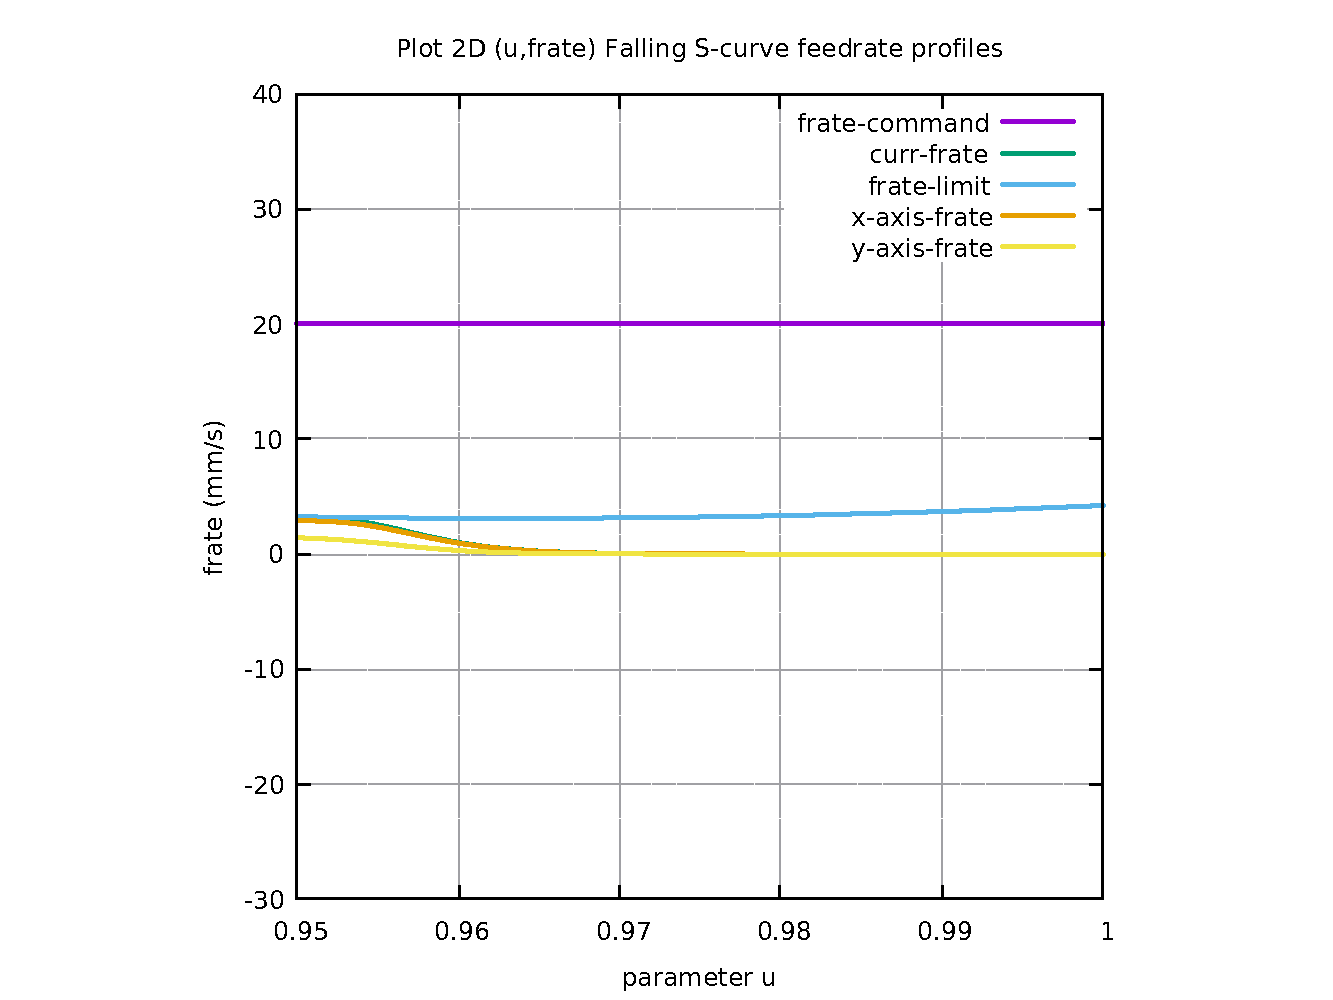
\includegraphics[width=1.00\textwidth]{Chap4/appendix/app-AstEpi/plots/16-img-AstEpi-FC20-Nominal-Falling-S-Curve-Profile.pdf}
\end{figure}

%% ==================================================
\clearpage
\pagebreak

\begin{figure}
	\caption     {AstEpi FC10 Colored Feedrate Profile data ngcode}
	\label{17-img-AstEpi-FC10-Colored-Feedrate-Profile-data_ngcode.png}
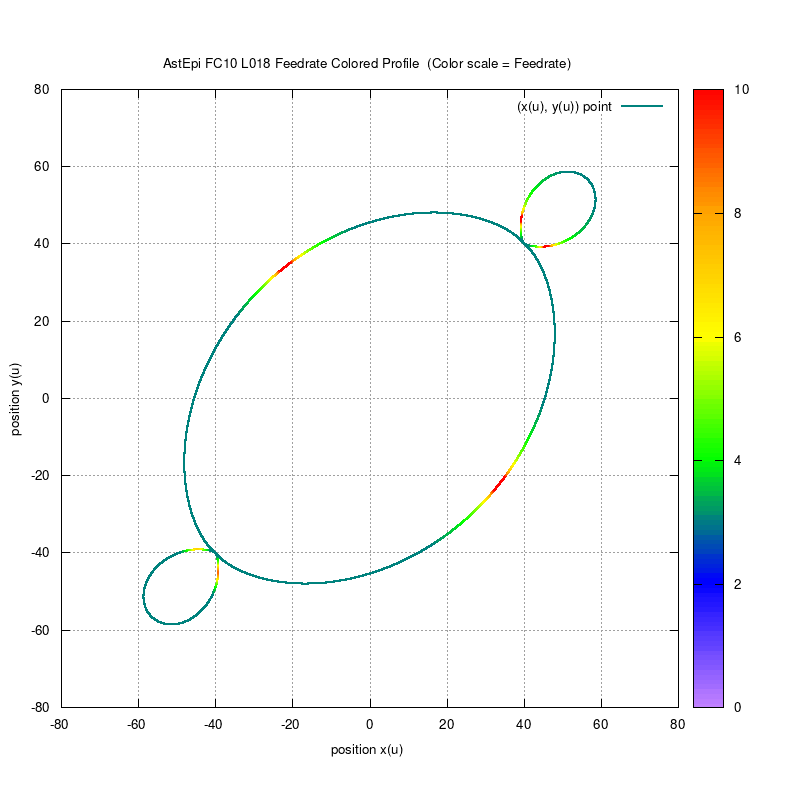
\includegraphics[width=0.75\textwidth]{Chap4/appendix/app-AstEpi/plots/17-img-AstEpi-FC10-Colored-Feedrate-Profile-data_ngcode.png}
\end{figure}


\begin{figure}
	\caption     {AstEpi FC20 Colored Feedrate Profile data ngcode}
	\label{18-img-AstEpi-FC20-Colored-Feedrate-Profile-data_ngcode.png}
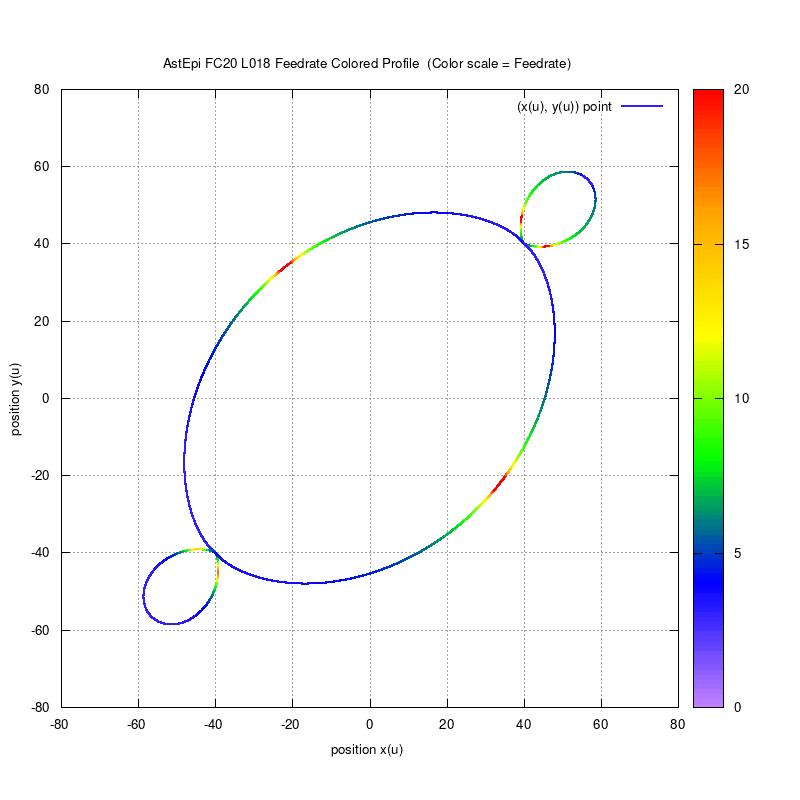
\includegraphics[width=0.75\textwidth]{Chap4/appendix/app-AstEpi/plots/18-img-AstEpi-FC20-Colored-Feedrate-Profile-data_ngcode.png}
\end{figure}

%% ==================================================
\clearpage
\pagebreak

\begin{figure}
	\caption     {AstEpi FC30 Colored Feedrate Profile data ngcode}
	\label{19-img-AstEpi-FC30-Colored-Feedrate-Profile-data_ngcode.png}
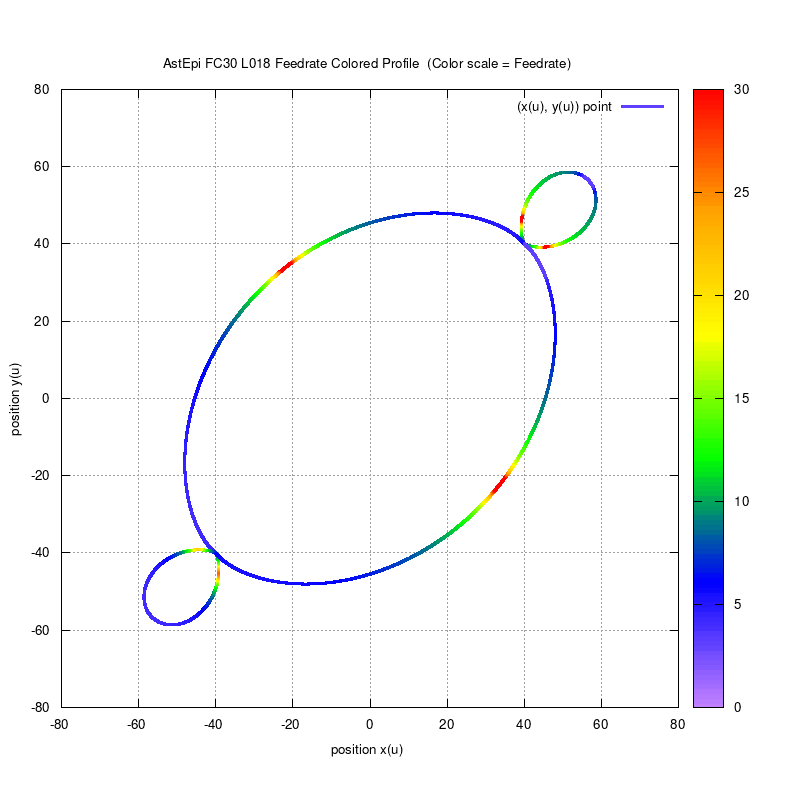
\includegraphics[width=0.75\textwidth]{Chap4/appendix/app-AstEpi/plots/19-img-AstEpi-FC30-Colored-Feedrate-Profile-data_ngcode.png}
\end{figure}


\begin{figure}
	\caption     {AstEpi FC40 Colored Feedrate Profile data ngcode}
	\label{20-img-AstEpi-FC40-Colored-Feedrate-Profile-data_ngcode.png}
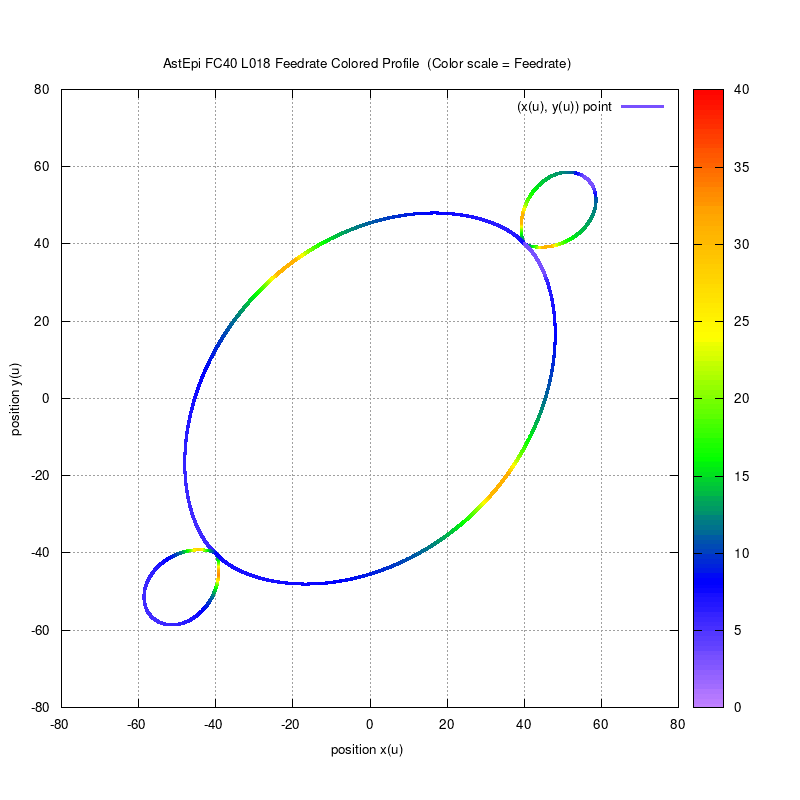
\includegraphics[width=0.75\textwidth]{Chap4/appendix/app-AstEpi/plots/20-img-AstEpi-FC40-Colored-Feedrate-Profile-data_ngcode.png}
\end{figure}

%% ==================================================
\clearpage
\pagebreak

\begin{figure}
	\caption     {AstEpi FC10 Tangential Acceleration}
	\label{21-img-AstEpi-FC10-Tangential-Acceleration.pdf}
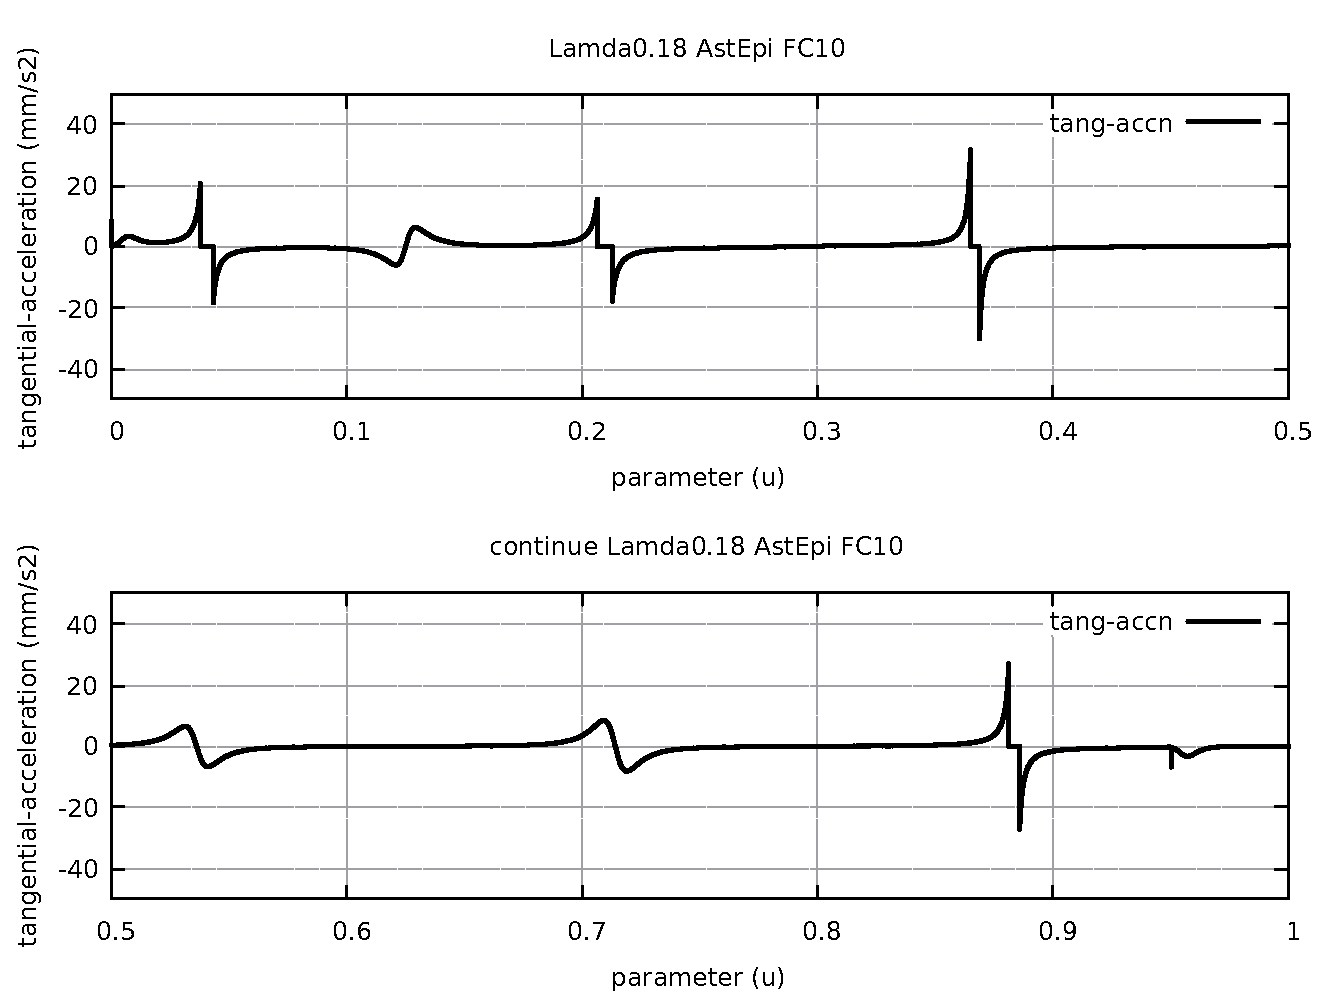
\includegraphics[width=1.00\textwidth]{Chap4/appendix/app-AstEpi/plots/21-img-AstEpi-FC10-Tangential-Acceleration.pdf}
\end{figure}


\begin{figure}
	\caption     {AstEpi FC20 Tangential Acceleration}
	\label{22-img-AstEpi-FC20-Tangential-Acceleration.pdf}
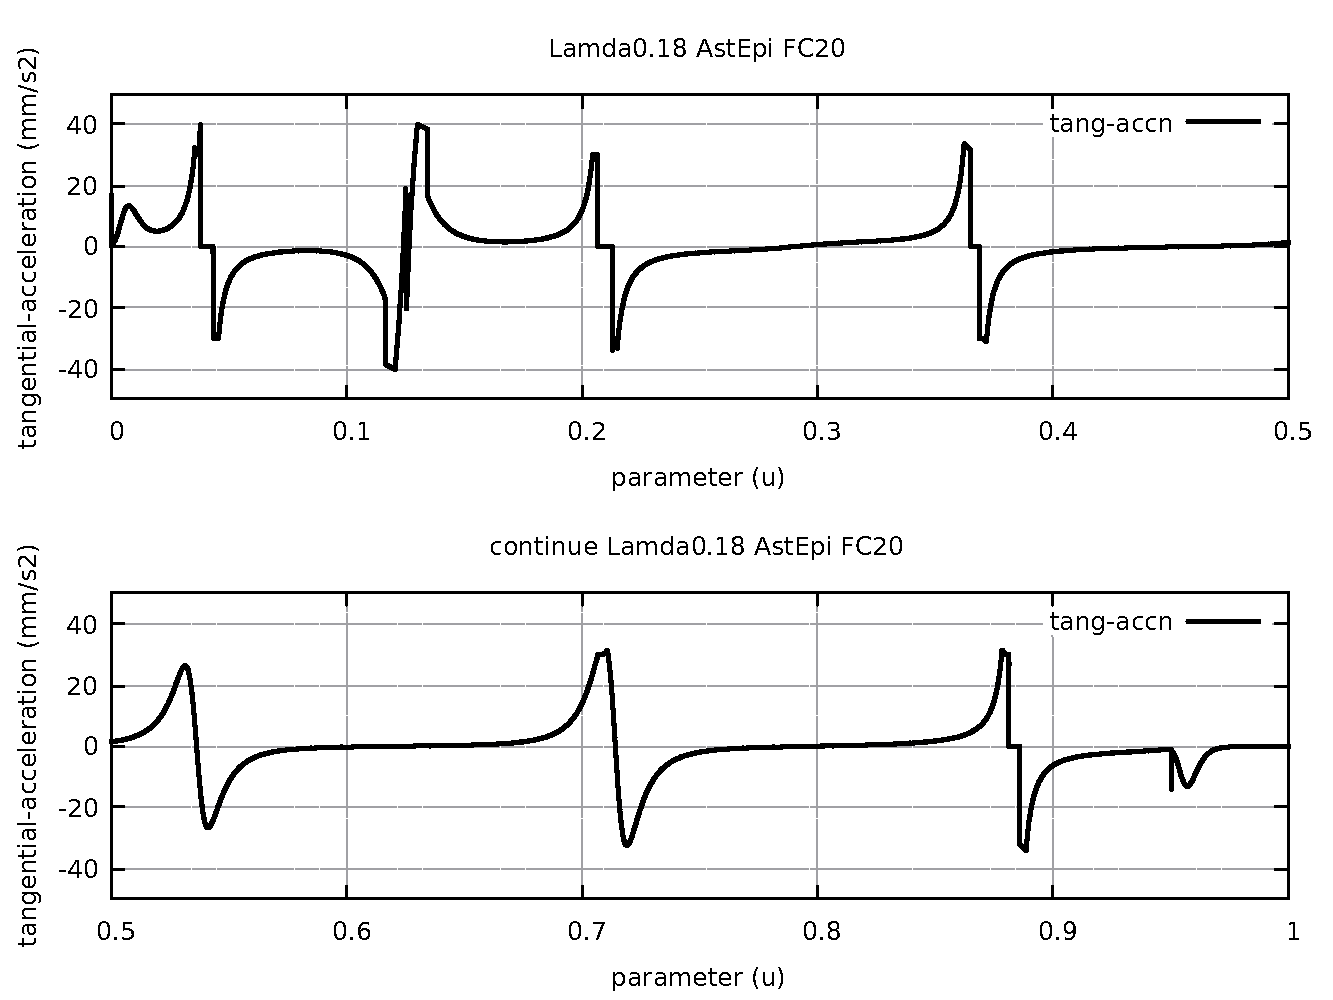
\includegraphics[width=1.00\textwidth]{Chap4/appendix/app-AstEpi/plots/22-img-AstEpi-FC20-Tangential-Acceleration.pdf}
\end{figure}

%% ==================================================
\clearpage
\pagebreak

\begin{figure}
	\caption     {AstEpi FC30 Tangential Acceleration}
	\label{23-img-AstEpi-FC30-Tangential-Acceleration.pdf}
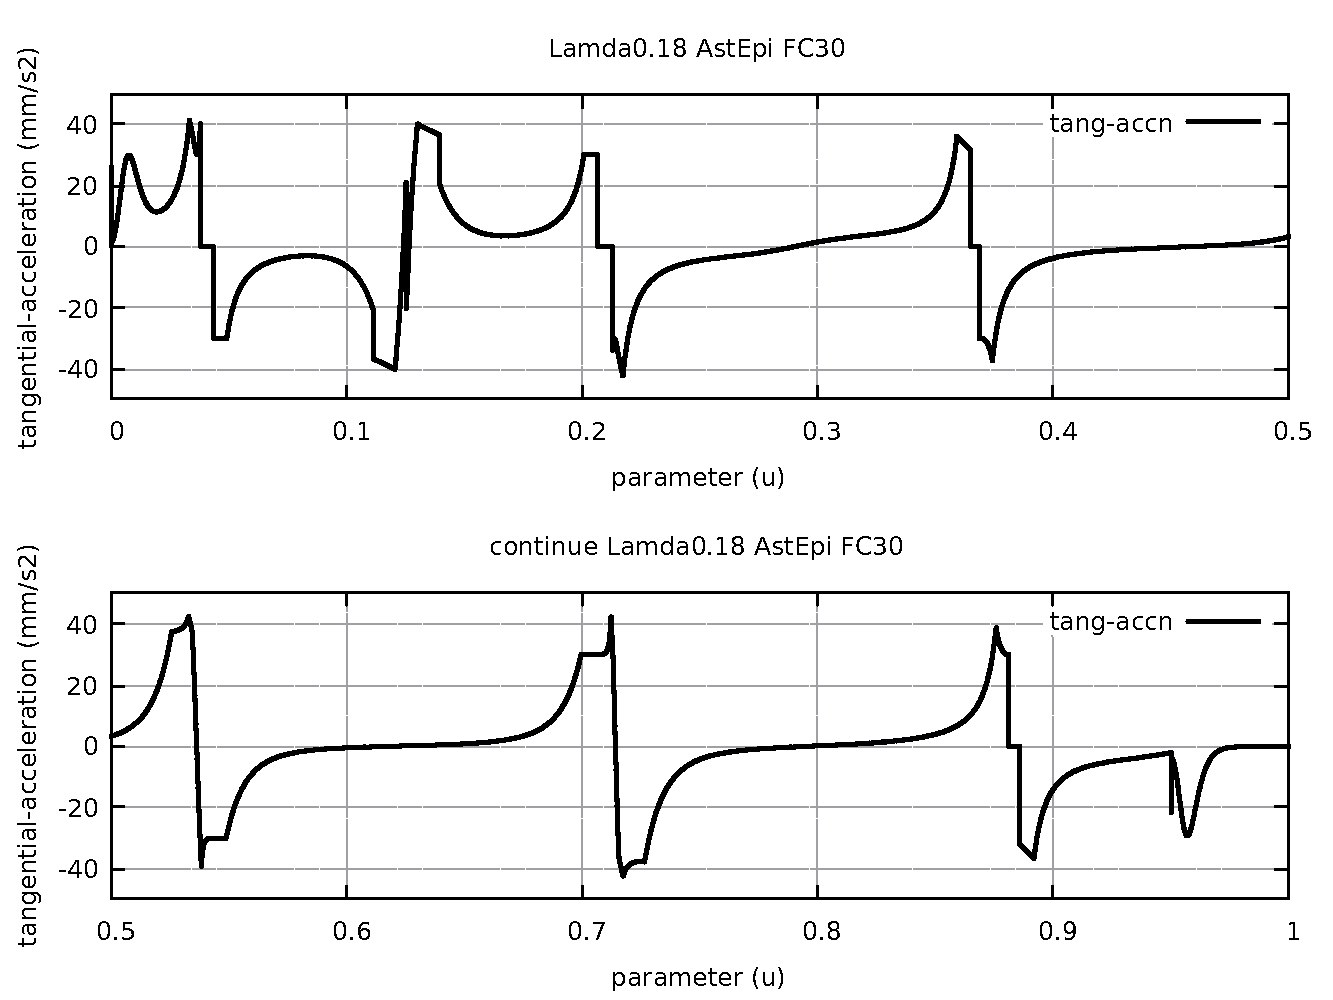
\includegraphics[width=1.00\textwidth]{Chap4/appendix/app-AstEpi/plots/23-img-AstEpi-FC30-Tangential-Acceleration.pdf}
\end{figure}


\begin{figure}
	\caption     {AstEpi FC40 Tangential Acceleration}
	\label{24-img-AstEpi-FC40-Tangential-Acceleration.pdf}
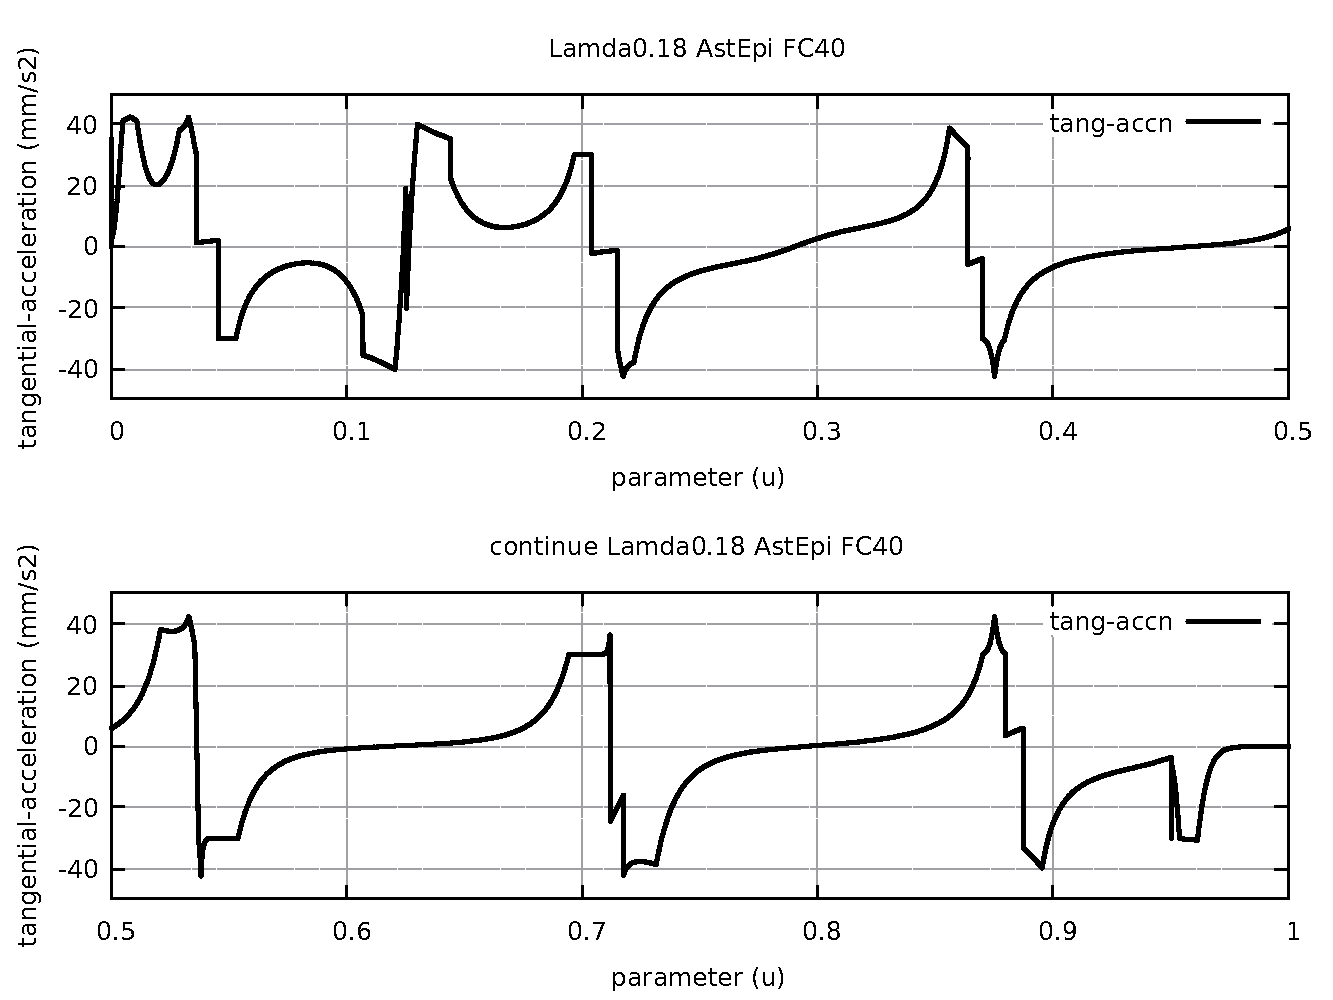
\includegraphics[width=1.00\textwidth]{Chap4/appendix/app-AstEpi/plots/24-img-AstEpi-FC40-Tangential-Acceleration.pdf}
\end{figure}

%% ==================================================
\clearpage
\pagebreak

\begin{figure}
	\caption     {AstEpi FC20 Nominal Separation NAL and NCL}
	\label{25-img-AstEpi-FC20-Nominal-Separation-NAL-and-NCL.pdf}
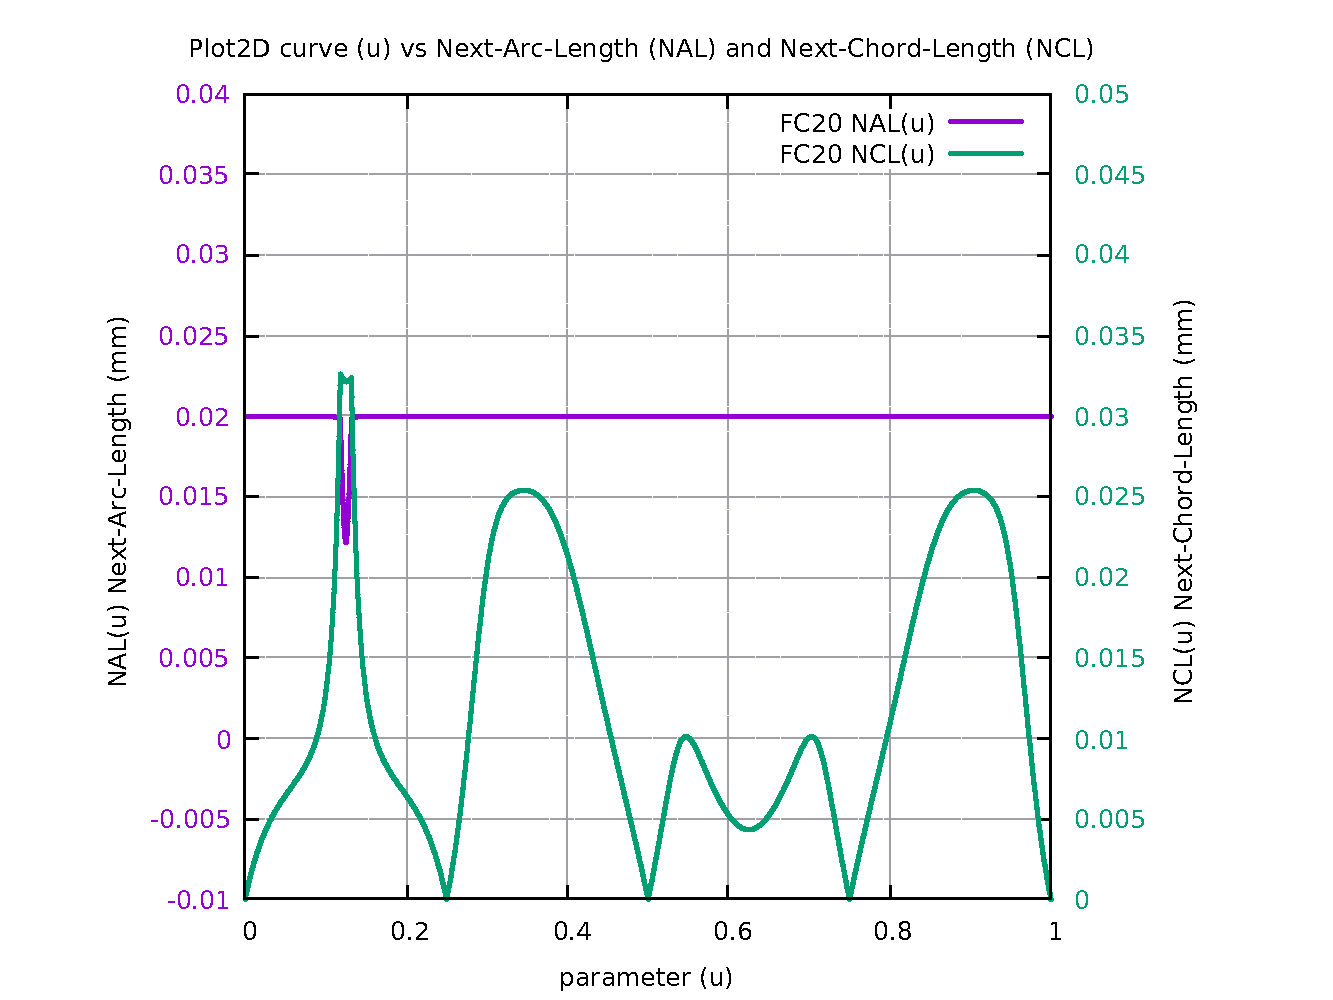
\includegraphics[width=1.00\textwidth]{Chap4/appendix/app-AstEpi/plots/25-img-AstEpi-FC20-Nominal-Separation-NAL-and-NCL.pdf}
\end{figure}


\begin{figure}
	\caption     {AstEpi Difference SAL minus SCL for FC10 FC20 FC30 FC40}
	\label{26-img-AstEpi-Difference-SAL-minus-SCL-for-FC10-FC20-FC30-FC40.pdf}
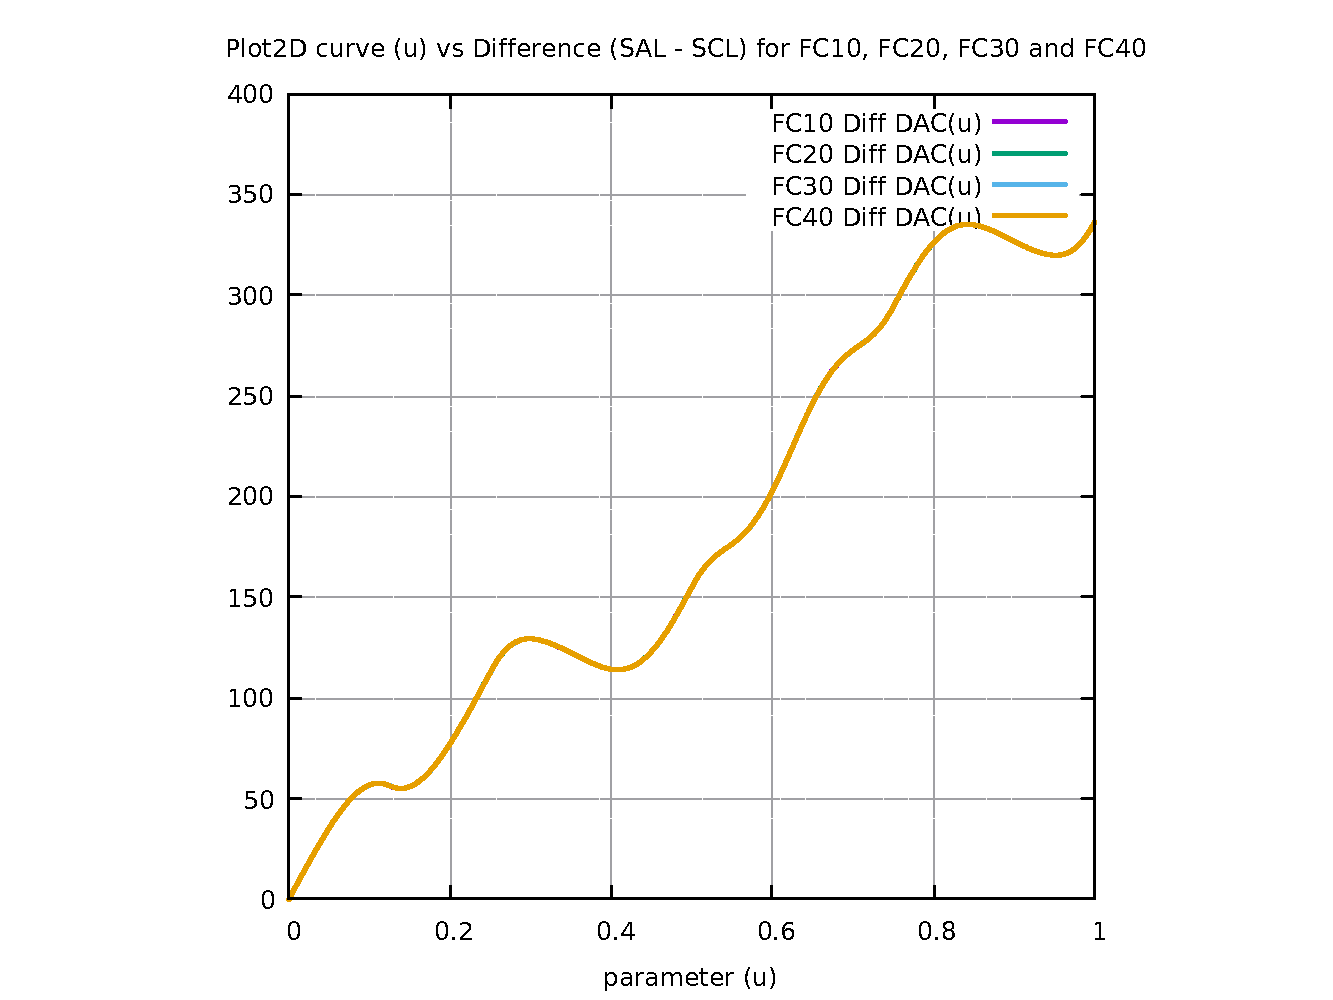
\includegraphics[width=1.00\textwidth]{Chap4/appendix/app-AstEpi/plots/26-img-AstEpi-Difference-SAL-minus-SCL-for-FC10-FC20-FC30-FC40.pdf}
\end{figure}


%% ==================================================
\clearpage
\pagebreak

\begin{figure}
	\caption     {AstEpi FC10 FrateCmd CurrFrate X-Frate Y-Frate}
	\label{27-img-AstEpi-FC10-FrateCmd-CurrFrate-X-Frate-Y-Frate.pdf}
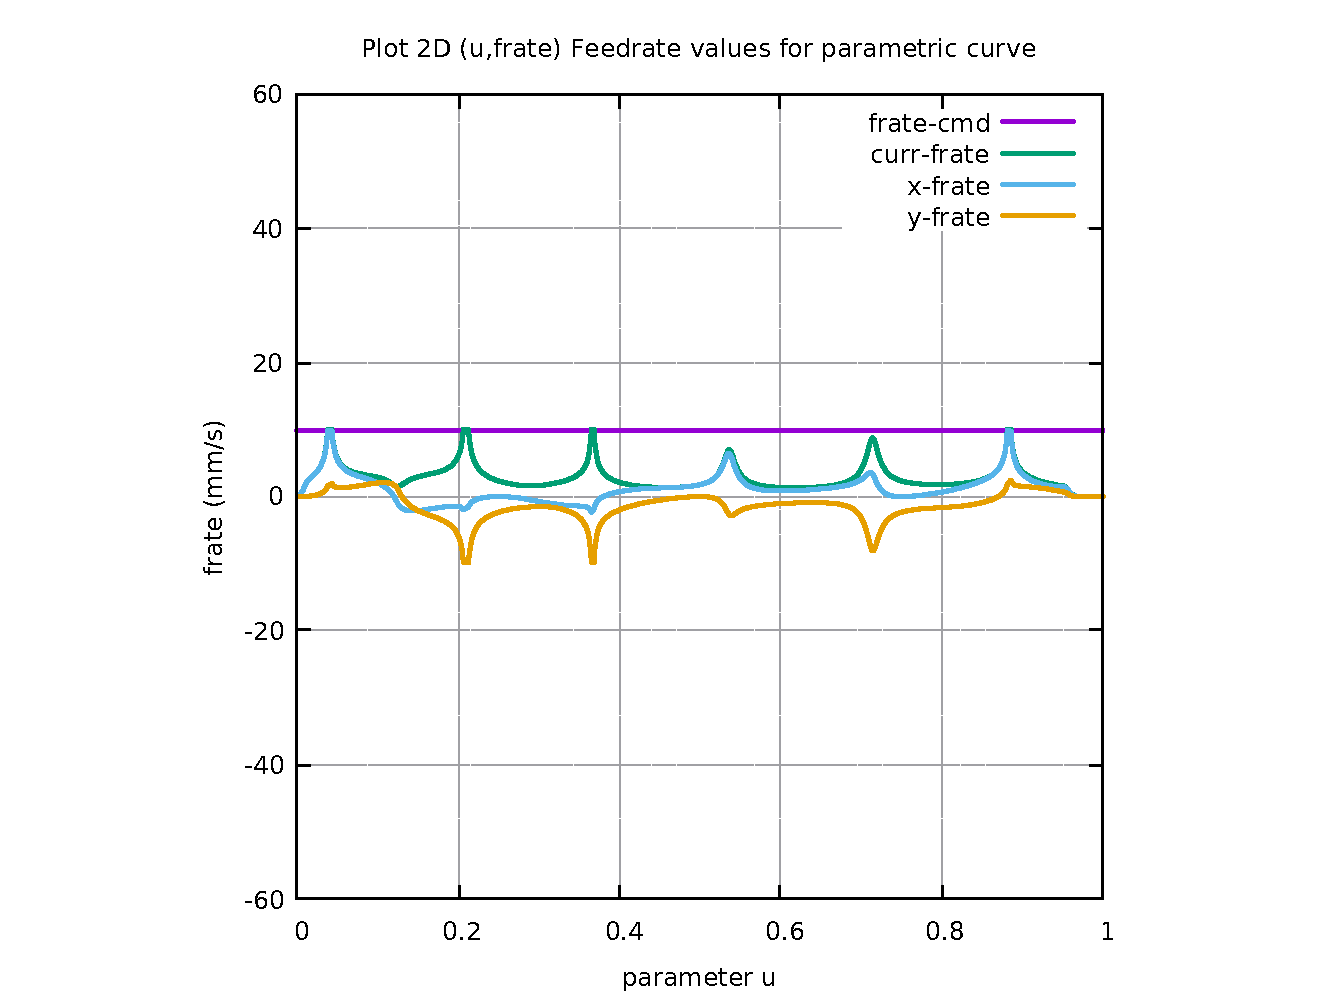
\includegraphics[width=1.00\textwidth]{Chap4/appendix/app-AstEpi/plots/27-img-AstEpi-FC10-FrateCmd-CurrFrate-X-Frate-Y-Frate.pdf}
\end{figure}


\begin{figure}
	\caption     {AstEpi FC20 FrateCmd CurrFrate X-Frate Y-Frate}
	\label{28-img-AstEpi-FC20-FrateCmd-CurrFrate-X-Frate-Y-Frate.pdf}
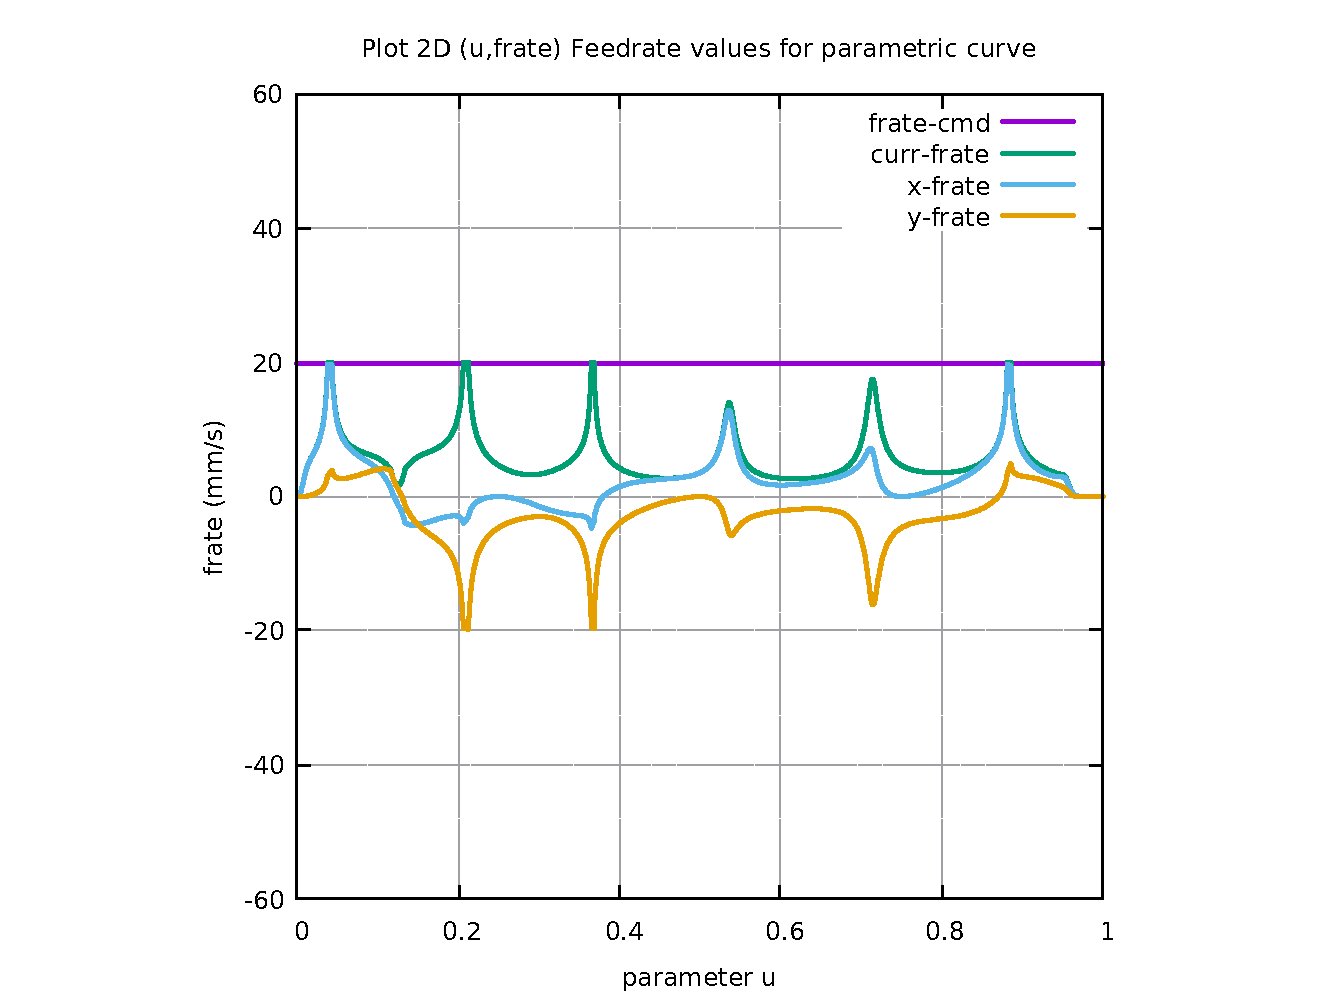
\includegraphics[width=1.00\textwidth]{Chap4/appendix/app-AstEpi/plots/28-img-AstEpi-FC20-FrateCmd-CurrFrate-X-Frate-Y-Frate.pdf}
\end{figure}


%% ==================================================
\clearpage
\pagebreak

\begin{figure}
	\caption     {AstEpi FC30 FrateCmd CurrFrate X-Frate Y-Frate}
	\label{29-img-AstEpi-FC30-FrateCmd-CurrFrate-X-Frate-Y-Frate.pdf}
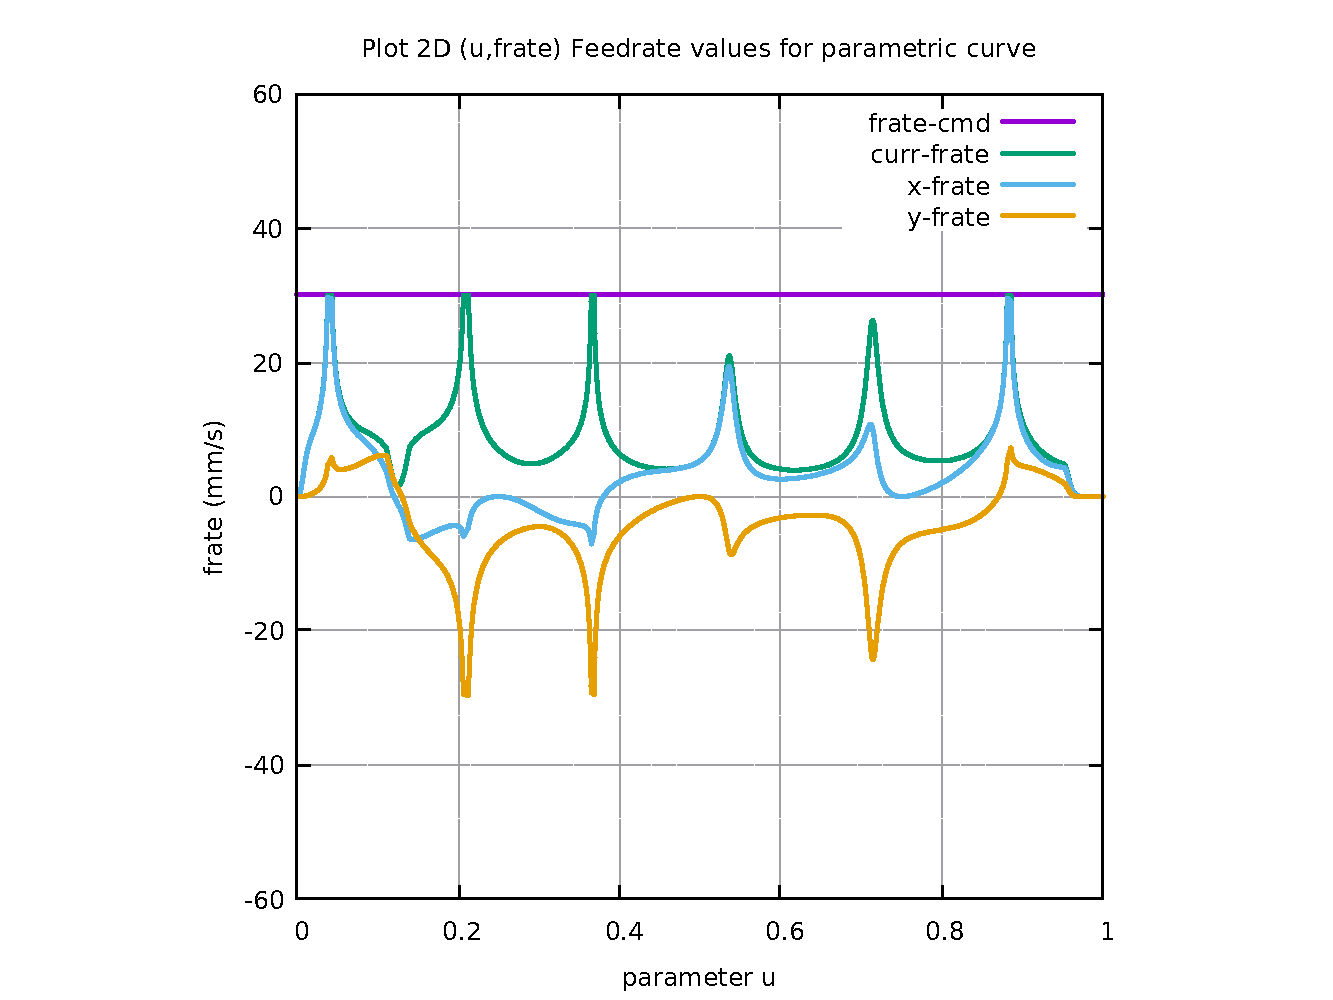
\includegraphics[width=1.00\textwidth]{Chap4/appendix/app-AstEpi/plots/29-img-AstEpi-FC30-FrateCmd-CurrFrate-X-Frate-Y-Frate.pdf}
\end{figure}


\begin{figure}
	\caption     {AstEpi FC40 FrateCmd CurrFrate X-Frate Y-Frate}
	\label{30-img-AstEpi-FC40-FrateCmd-CurrFrate-X-Frate-Y-Frate.pdf}
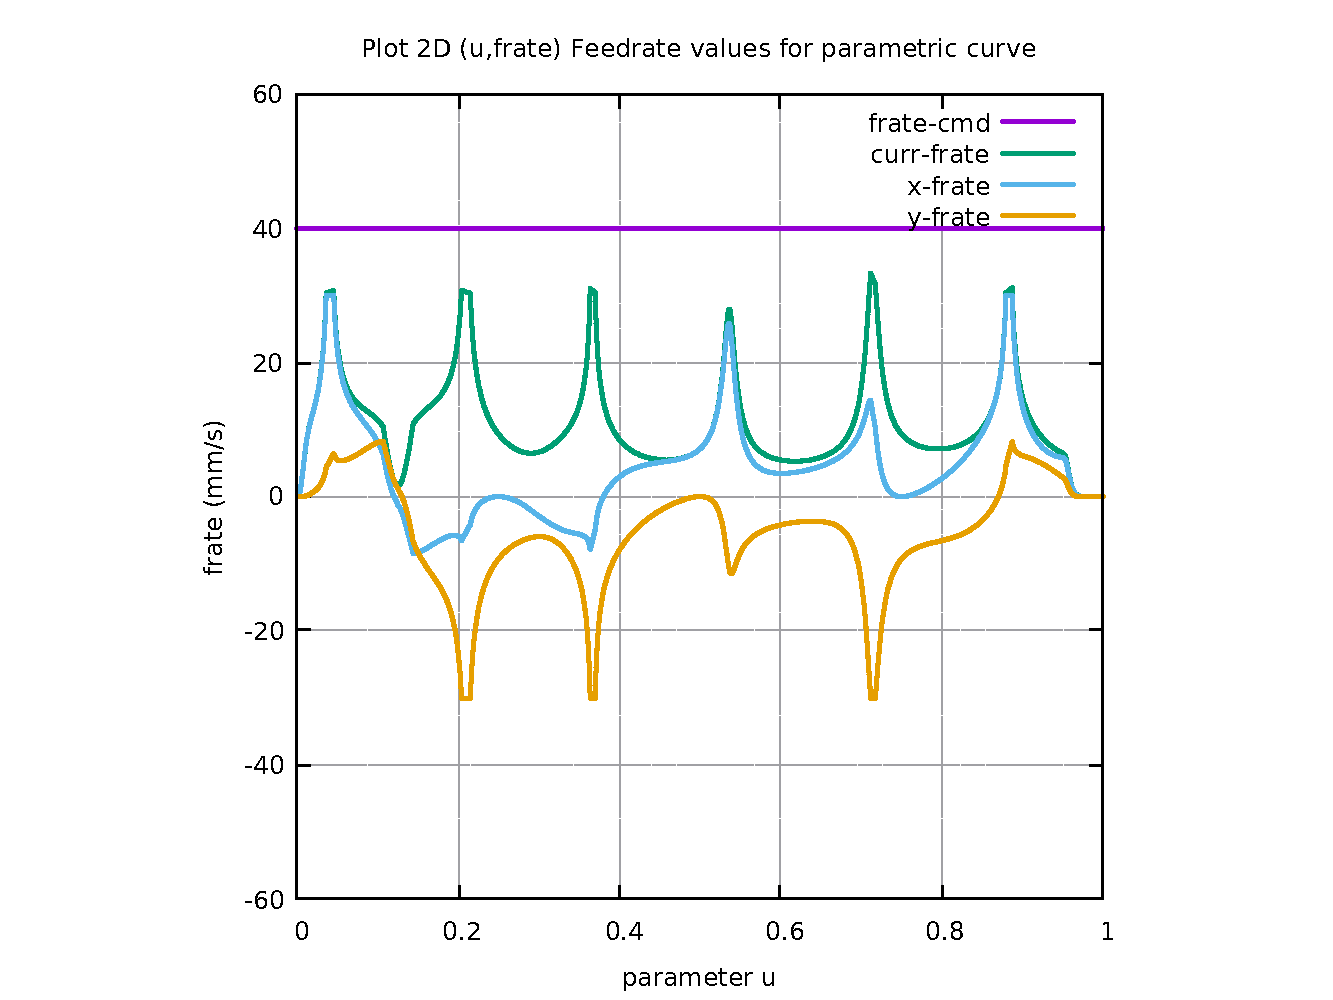
\includegraphics[width=1.00\textwidth]{Chap4/appendix/app-AstEpi/plots/30-img-AstEpi-FC40-FrateCmd-CurrFrate-X-Frate-Y-Frate.pdf}
\end{figure}


%% ==================================================
\clearpage
\pagebreak

\begin{figure}
	\caption     {AstEpi FC10 Four Components FeedrateLimit}
	\label{31-img-AstEpi-FC10-Four-Components-FeedrateLimit.pdf}
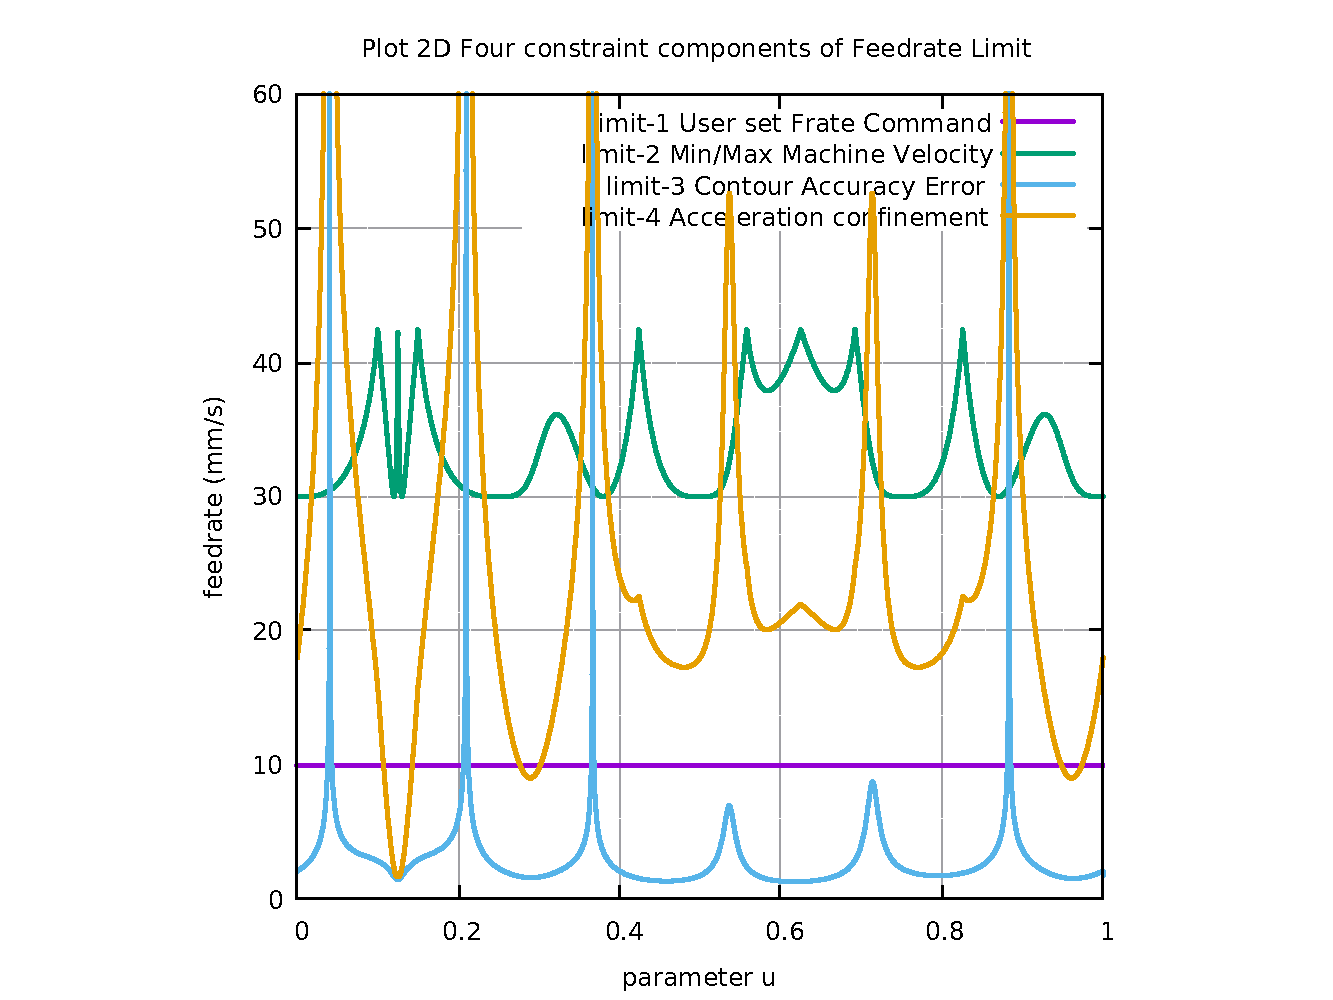
\includegraphics[width=1.00\textwidth]{Chap4/appendix/app-AstEpi/plots/31-img-AstEpi-FC10-Four-Components-FeedrateLimit.pdf}
\end{figure}


\begin{figure}
	\caption     {AstEpi FC20 Four Components FeedrateLimit}
	\label{32-img-AstEpi-FC20-Four-Components-FeedrateLimit.pdf}
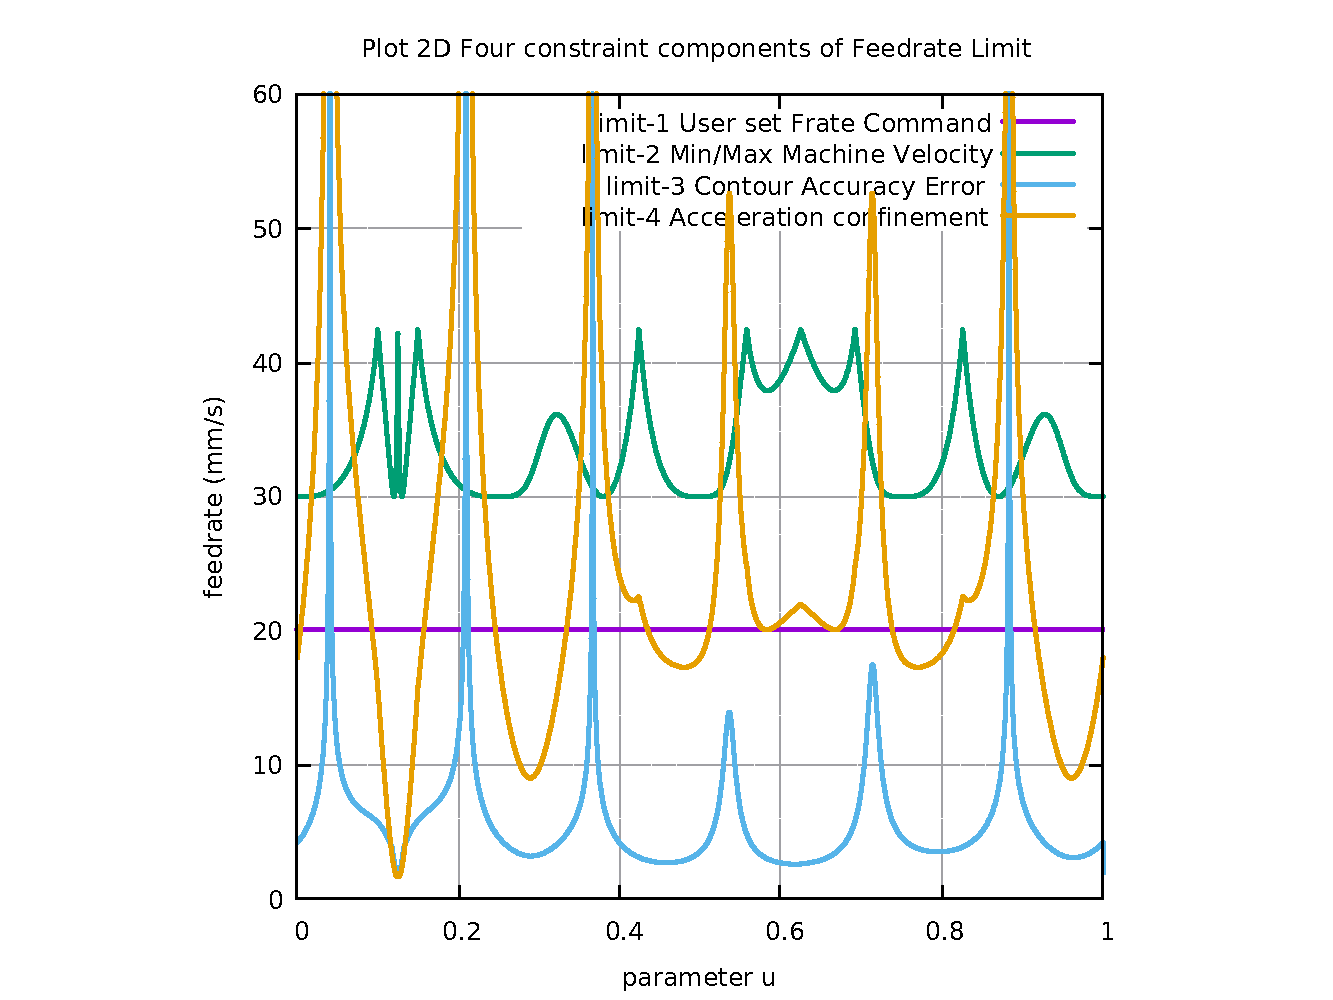
\includegraphics[width=1.00\textwidth]{Chap4/appendix/app-AstEpi/plots/32-img-AstEpi-FC20-Four-Components-FeedrateLimit.pdf}
\end{figure}


%% ==================================================
\clearpage
\pagebreak

\begin{figure}
	\caption     {AstEpi FC30 Four Components FeedrateLimit}
	\label{33-img-AstEpi-FC30-Four-Components-FeedrateLimit.pdf}
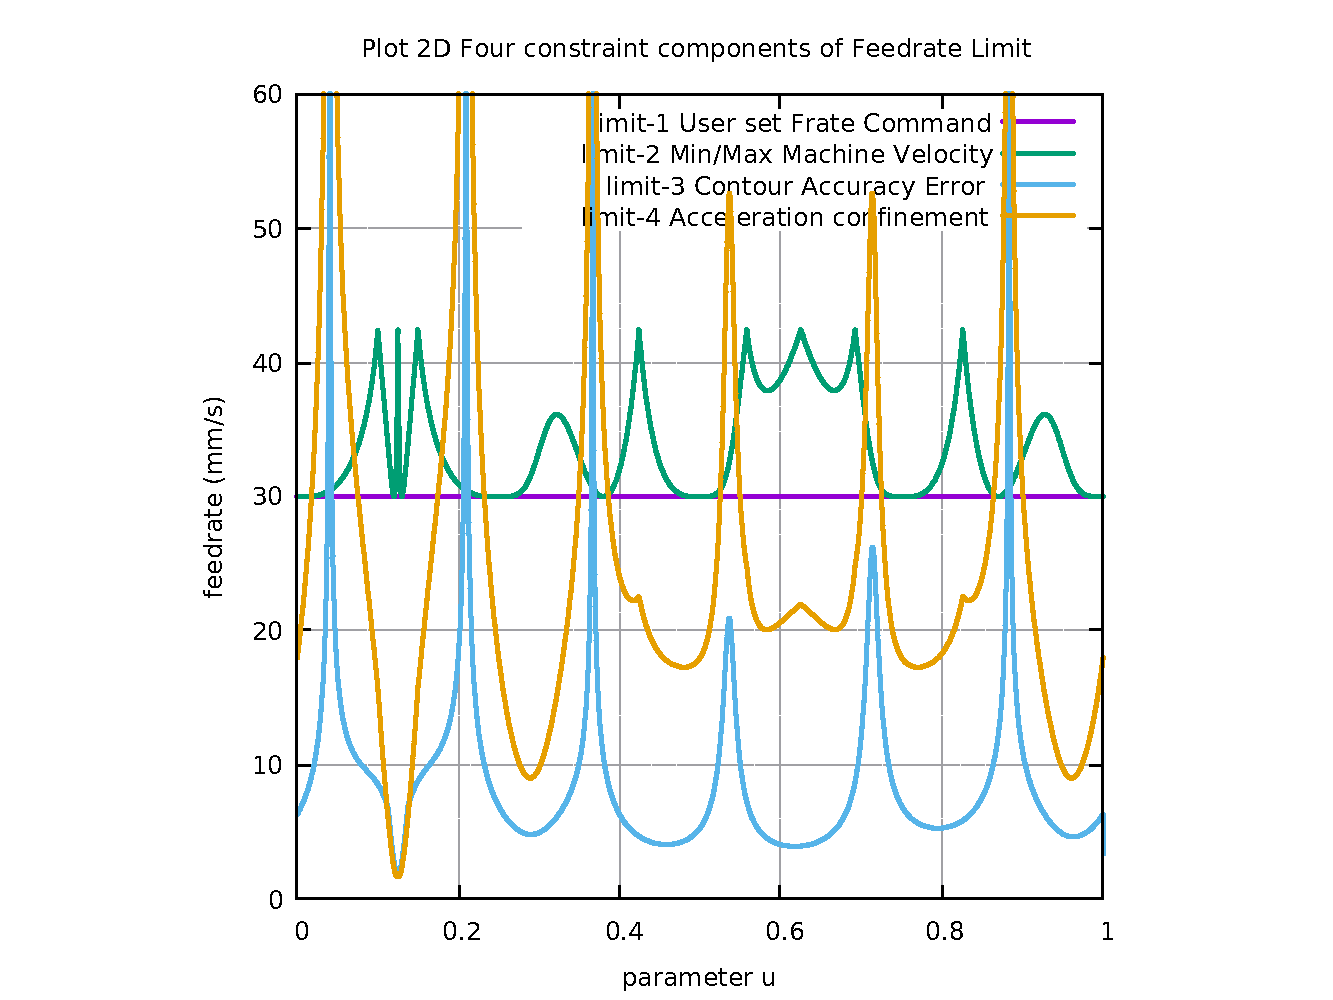
\includegraphics[width=1.00\textwidth]{Chap4/appendix/app-AstEpi/plots/33-img-AstEpi-FC30-Four-Components-FeedrateLimit.pdf}
\end{figure}


\begin{figure}
	\caption     {AstEpi FC40 Four Components FeedrateLimit}
	\label{34-img-AstEpi-FC40-Four-Components-FeedrateLimit.pdf}
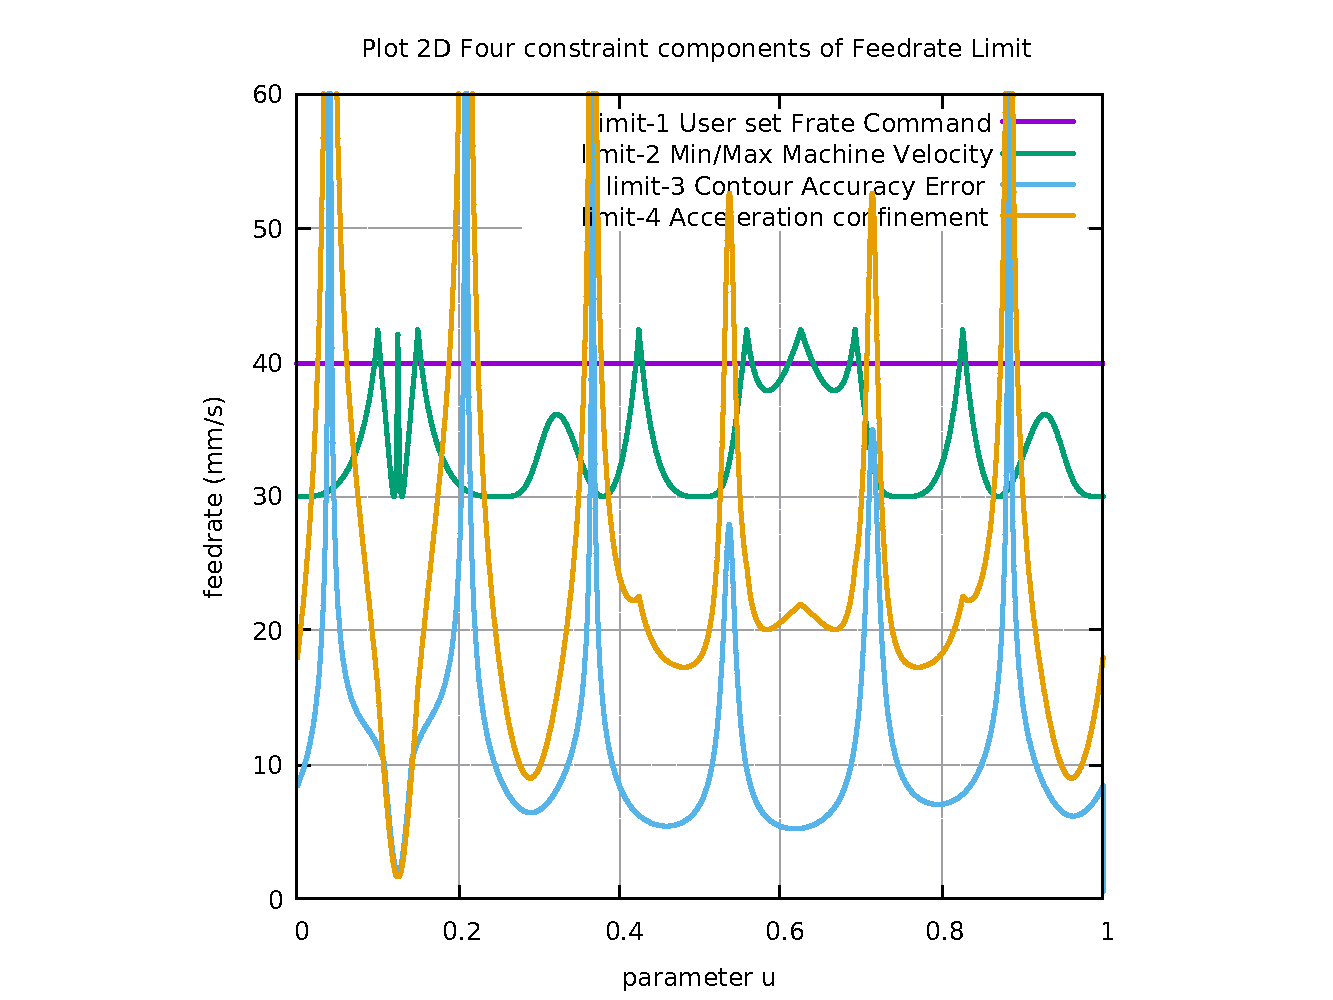
\includegraphics[width=1.00\textwidth]{Chap4/appendix/app-AstEpi/plots/34-img-AstEpi-FC40-Four-Components-FeedrateLimit.pdf}
\end{figure}


%% =======================================
\clearpage
\pagebreak

\begin{figure}
	\centering
	\caption     {AstEpi Histogram Points FC10 FC20 FC30 FC40}
	\label{35-img-AstEpi-Histogram-Points-FC10-FC20-FC30-FC40.pdf}
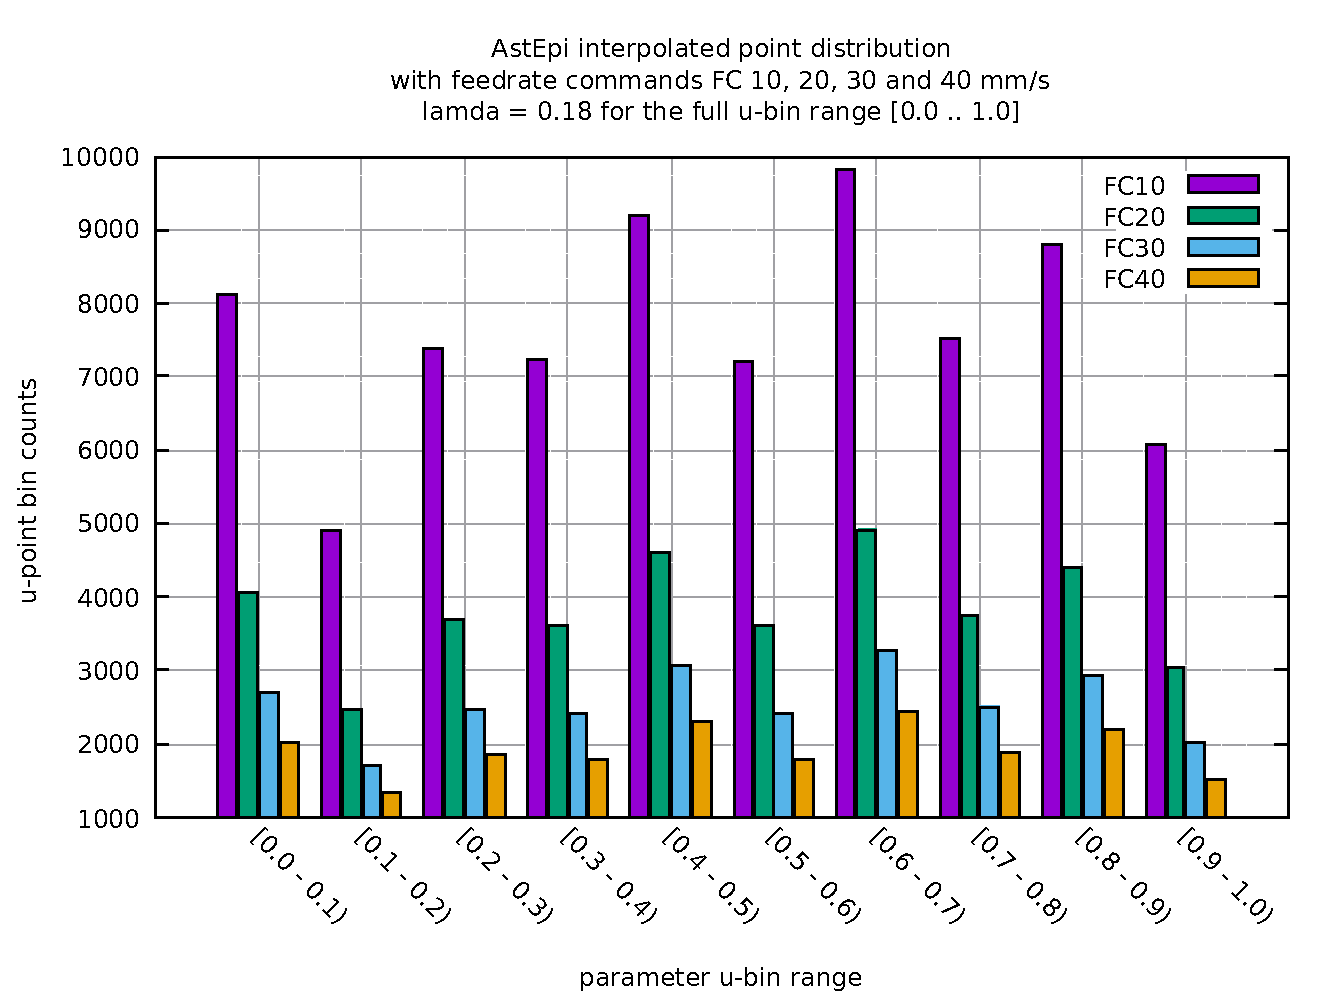
\includegraphics[width=1.00\textwidth]{Chap4/appendix/app-AstEpi/plots/35-img-AstEpi-Histogram-Points-FC10-FC20-FC30-FC40.pdf} 
\end{figure}


\begin{table}[ht]
%% \begin{center}
\caption    {AstEpi Table distribution of interpolated points}
\label  {tab-AstEpi Table distribution of interpolated points}
	
%% IMPORTANT TO SCALEBOX BELOW
\scalebox{0.80}{
		
%% START COPY AND PASTE BELOW HERE
%% FROM \begin{tabular} UNTIL \end{tabular)
%% Note: adjust last p{} to get line width correct
		
\begin{tabular}{ p{4.5cm} p{1.5cm} p{1.5cm} p{1.5cm} p{7.50cm} }
\hline
	&		&		&		&		\\
BINS	&	FC10	&	FC20	&	FC30	&	FC40	\\
&		&		&		&		\\
0.0 - 0.1	&	8110	&	4055	&	2704	&	2028	\\
0.1 - 0.2	&	4901	&	2478	&	1702	&	1334	\\
0.2 - 0.3	&	7391	&	3696	&	2464	&	1848	\\
0.3 - 0.4	&	7234	&	3617	&	2412	&	1809	\\
0.4 - 0.5	&	9182	&	4592	&	3061	&	2297	\\
0.5 - 0.6	&	7216	&	3608	&	2406	&	1804	\\
0.6 - 0.7	&	9831	&	4916	&	3278	&	2458	\\
0.7 - 0.8	&	7525	&	3763	&	2508	&	1882	\\
0.8 - 0.9	&	8801	&	4401	&	2935	&	2201	\\
0.9 - 1.0	&	6084	&	3043	&	2029	&	1523	\\
&		&		&		&		\\
Tot Counts	&	76275	&	38169	&	25499	&	19184	\\
&		&		&		&		\\
\hline	
\end{tabular}
		
%% END COPY AND PASTE ABOVE HERE
		
}   %% IMPORTANT FOR SCALEBOX CLOSING
	
\end{table}
%% \end{landscape}

%% AstEpi SUMMARY TABLE
%% ========================================================
\clearpage
\pagebreak
\begin{landscape}
	
\begin{table}[ht]
%% \begin{center}
\caption       {AstEpi Table FC10-20-30-40 Run Performance data}
\label{tab-app4-AstEpi-Table-FC10-20-30-40-Run-Performance-data}
		
%% IMPORTANT TO SCALEBOX BELOW
\scalebox{0.90}{
			
%% START COPY AND PASTE BELOW HERE
%% FROM \begin{tabular} UNTIL \end{tabular)
			
			
\begin{tabular}{ p{0.2cm} p{8.80cm} p{4.00cm} p{4.0cm} p{4.00cm} p{4.0cm}}
	\hline
	&		&		&		&		&		\\
	1	&	Curve Type	&	ASTEPI	&	ASTEPI	&	ASTEPI	&	ASTEPI	\\
	2	&	User Feedrate Command FC(mm/s)                   	&	FC10	&	FC20	&	FC30	&	FC40	\\
	3	&	User Lamda Acceleration Safety Factor	&	0.18	&	0.18	&	0.18	&	0.18	\\
	&		&		&		&		&		\\
	4	&	Total Iterpolated Points (TIP)	&	76275	&	38169	&	25499	&	19184	\\
	5	&	Total Sum-Chord-Error (SCE) (mm)	&	8.403732211685E-04	&	1.641842648547E-03	&	2.390002467065E-03	&	3.111370462905E-03	\\
	6	&	Ratio 1 = (SCE/TIP) = Chord-Error/Point	&	1.101782024240E-08	&	4.301620856599E-08	&	9.373293854673E-08	&	1.621941543505E-07	\\
	&		&		&		&		&		\\
	7	&	Total Sum-Arc-Length (SAL) (mm)	&	7.626471894183E+02	&	7.626564180797E+02	&	7.626597716718E+02	&	7.626830175974E+02	\\
	8	&	Total Sum-Chord-Length (SCL) (mm)	&	4.262622478423E+02	&	4.262622396899E+02	&	4.262622295515E+02	&	4.262622333550E+02	\\
	9	&	Difference = (SAL – SCL) (mm)	&	3.363849415760E+02	&	3.363941783897E+02	&	3.363975421203E+02	&	3.364207842424E+02	\\
	10	&	Percentage Difference = (SAL – SCL)/SAL	&	4.410754359858E+01	&	4.410822100426E+01	&	4.410846810274E+01	&	4.411017113009E+01	\\
	&		&		&		&		&		\\
	11	&	Ratio 2 = (SCE/SCL) = Chord Error/Chord-Length	&	1.971493430212E-06	&	3.851719659103E-06	&	5.606883043752E-06	&	7.299193359018E-06	\\
	&		&		&		&		&		\\
	12	&	Total Sum-Arc-Theta (SAT) (rad)	&	1.300410711943E+01	&	1.300415390419E+01	&	1.300401093322E+01	&	1.300396323193E+01	\\
	13	&	Total Sum-Arc-Area (SAA) (mm2)	&	2.898515736808E-04	&	6.811935608835E-04	&	9.367445601128E-04	&	1.255001527807E-03	\\
	&		&		&		&		&		\\
	14	&	Ratio 3 = (SAA/SCL) = Arc-Area/Chord-Length	&	1.971493430212E-06	&	3.851719659103E-06	&	5.606883043752E-06	&	7.299193359018E-06	\\
	&		&		&		&		&		\\
	15	&	Average-Chord-Error (ACE) (mm)	&	1.101782024240E-08	&	4.301620856599E-08	&	9.373293854673E-08	&	1.621941543505E-07	\\
	16	&	Average-Arc-Length (AAL) (mm)	&	9.998783195037E-03	&	1.998156618318E-02	&	2.991057226731E-02	&	3.975827647383E-02	\\
	17	&	Average-Chord-Length (ACL) (mm)	&	5.588565537959E-03	&	1.116805281099E-02	&	1.671747703944E-02	&	2.222083268285E-02	\\
	18	&	Average-Arc-Theta (AAT) (rad)	&	1.704920040831E-04	&	3.407082871566E-04	&	5.100012131627E-04	&	6.778899667376E-04	\\
	19	&	Average-Arc-Area (AAA) (mm2)	&	3.800136005465E-09	&	1.784724273956E-08	&	3.673796219754E-08	&	6.542258915741E-08	\\
	&		&		&		&		&		\\
	20	&	Algorithm actual runtime on computer (ART) (s) 	&	27.836373672	&	14.372286925	&	9.138001576	&	7.71877336	\\
	&		&		&		&		&		\\
	\hline
\end{tabular}

			
%% END COPY AND PASTE		
}   %% IMPORTANT FOR SCALEBOX CLOSING
		
\end{table}
\end{landscape}

%% =======================================
\clearpage
\pagebreak
